\documentclass[12pt]{article}%
%%%%%%%%%%%%%%%%%%%%%%%%%%%%%%%%%%%%%%%%%%%%%%%%%%%%%%%%%%%%%%%%%   
% All style files are available from 
%   http://wwww.uiuc.edu/~sariel/research/latex/
%%%%%%%%%%%%%%%%%%%%%%%%%%%%%%%%%%%%%%%%%%%%%%%%%%%%%%%%%%%%%%%%%%   


%%%%%%%%%%%%%%%%%%%%%%%%%%%%%%%%%%%%%%%%%%%%%%%%%%%%%%%%%%%%%%%%%%   
% Conditional compilation depending on whether this is my computer or
% not.
\IfFileExists{sariel_computer.sty}{\def\sarielComp{1}}{}
\ifx\sarielComp\undefined%
\newcommand{\SarielComp}[1]{}
\newcommand{\NotSarielComp}[1]{#1}%
\else
\newcommand{\SarielComp}[1]{#1}%
\newcommand{\NotSarielComp}[1]{}%
\fi
\newcommand{\IfPrinterVer}[2]{#2}%

%%%%%%%%%%%%%%%%%%%%%%%%%%%%%%%%%%%%%%%%%%%%%%%%%%%%%%%%%%%%%%%%%% 


\usepackage[cm]{fullpage}%
\usepackage{amsmath}%
\usepackage{amssymb}%
\usepackage[cmyk]{xcolor}%
%\usepackage{xcolor}%

\SarielComp{\usepackage{sariel_colors}}%

\usepackage[amsmath,thmmarks]{ntheorem}%
\theoremseparator{.}%

\usepackage{titlesec}%
\titlelabel{\thetitle. }%

\usepackage{graphicx}%
\usepackage{xcolor}%
\usepackage{mleftright}%
\usepackage{xspace}%
\usepackage{hyperref}%

\usepackage{caption}%

\newcommand{\hrefb}[3][black]{\href{#2}{\color{#1}{#3}}}%

\IfPrinterVer{%
   \usepackage{hyperref}%
}{%
   \usepackage{hyperref}%
   \hypersetup{%
      breaklinks,%
      ocgcolorlinks, colorlinks=true,%
      urlcolor=[rgb]{0.25,0.0,0.0},%
      linkcolor=[rgb]{0.5,0.0,0.0},%
      citecolor=[rgb]{0,0.2,0.445},%
      filecolor=[rgb]{0,0,0.4},
      anchorcolor=[rgb]={0.0,0.1,0.2}%
   }
   % \usepackage{cleveref}
}

% ----------------------------------------------------------------------
% ----------------------------------------------------------------------
% Defining theorem like environments
% ----------------------------------------------------------------------
% ----------------------------------------------------------------------
\theoremseparator{.}%

\theoremstyle{plain}%
\newtheorem{theorem}{Theorem}[section]

\newtheorem{lemma}[theorem]{Lemma}
\newtheorem{conjecture}[theorem]{Conjecture}
\newtheorem{corollary}[theorem]{Corollary}
\newtheorem{claim}[theorem]{Claim}%
\newtheorem{fact}[theorem]{Fact}
\newtheorem{observation}[theorem]{Observation}
\newtheorem{invariant}[theorem]{Invariant}
\newtheorem{question}[theorem]{Question}
\newtheorem{proposition}[theorem]{Proposition}
\newtheorem{prop}[theorem]{Proposition}
\newtheorem{openproblem}[theorem]{Open Problem}

\theoremstyle{plain}%
\theoremheaderfont{\sf} \theorembodyfont{\upshape}%
\newtheorem*{remark:unnumbered}[theorem]{Remark}%
\newtheorem*{remarks}[theorem]{Remarks}%
\newtheorem{remark}[theorem]{Remark}%
\newtheorem{definition}[theorem]{Definition}
\newtheorem{defn}[theorem]{Definition}
\newtheorem{example}[theorem]{Example}
\newtheorem{exercise}[theorem]{Exercise}
\newtheorem{problem}[theorem]{Problem}
\newtheorem{xca}[theorem]{Exercise}
\newtheorem{exercise_h}[theorem]{Exercise}
\newtheorem{assumption}[theorem]{Assumption}%

% Proof environment
\newcommand{\myqedsymbol}{\rule{2mm}{2mm}}

\theoremheaderfont{\em}%
\theorembodyfont{\upshape}%
\theoremstyle{nonumberplain}%
\theoremseparator{}%
\theoremsymbol{\myqedsymbol}%
\newtheorem{proof}{Proof:}%

\newtheorem{proofof}{Proof of\!}%

% theorem block end
%%%%%%%%%%%%%%%%%%%%%%%%%%%%%%%%%%%%%%%%%%%%%%%%%%%%%%%%%%%%%%%%%%%%


%%%%%%%%%%%%%%%%%%%%%%%%%%%%%%%%%%%%%%%%%%%%%%%%%%%%%%%%%%%%%%%%%% 5
% Color emph
\providecommand{\emphind}[1]{\emph{#1}\index{#1}}
\definecolor{nalmostblack}{rgb}{0, 0, 0.7}
\providecommand{\emphic}[2]{%
   \textcolor{nalmostblack}{%
      \textbf{\emph{#1}}}%
   \index{#2}}


\providecommand{\emphi}[1]{\emphic{#1}{#1}}

\definecolor{almostblack}{rgb}{0, 0, 0.5}
\providecommand{\emphw}[1]{{\emph{{\textcolor{almostblack}{#1}}}}}%

\providecommand{\emphOnly}[1]{\emph{\textcolor{almostblack}{\textbf{#1}}}}
% Color emph - end 
%%%%%%%%%%%%%%%%%%%%%%%%%%%%%%%%%%%%%%%%%%%%%%%%%%%%%%%%%%%%%%%%%% 5


\numberwithin{figure}{section}%
\numberwithin{table}{section}%
\numberwithin{equation}{section}%


%%%%%%%%%%%%%%%%%%%%%%%%%%%%%%%%%%%%%%%%%%%%%%%%%%%%%%%%%%%%%%%%%%%
% Sariel's thanks
%%%%%%%%%%%%%%%%%%%%%%%%%%%%%%%%%%%%%%%%%%%%%%%%%%%%%%%%%%%%%%%%%%% 

\providecommand{\tildegen}{{\protect\raisebox{-0.1cm}
      {\symbol{'176}\hspace{-0.01cm}}}}
\newcommand{\atgen}{\symbol{'100}}
\newcommand{\SarielThanks}[1]{\thanks{Department of Computer Science;
      University of Illinois; 201 N. Goodwin Avenue; Urbana, IL,
      61801, USA; {\tt sariel\atgen{}illinois.edu}; {\tt
         \url{http://sarielhp.org/}.} #1}}


%%%%%%%%%%%%%%%%%%%%%%%%%%%%%%%%%%%%%%%%%%%%%%%%%%%%%%%%%%%%%%%%%%%%%%
%    Handling references
%%%%%%%%%%%%%%%%%%%%%%%%%%%%%%%%%%%%%%%%%%%%%%%%%%%%%%%%%%%%%%%%%%%%%%

\newcommand{\HLink}[2]{\hyperref[#2]{#1~\ref*{#2}}}
\newcommand{\HLinkSuffix}[3]{\hyperref[#2]{#1\ref*{#2}{#3}}}

\newcommand{\figlab}[1]{\label{fig:#1}}
\newcommand{\figref}[1]{\HLink{Figure}{fig:#1}}

\newcommand{\thmlab}[1]{{\label{theo:#1}}}
\newcommand{\thmref}[1]{\HLink{Theorem}{theo:#1}}

\newcommand{\corlab}[1]{\label{cor:#1}}
\newcommand{\corref}[1]{\HLink{Corollary}{cor:#1}}%

\providecommand{\deflab}[1]{\label{def:#1}}
\newcommand{\defref}[1]{\HLink{Definition}{def:#1}}


\newcommand{\clmlab}[1]{\label{claim:#1}}
\newcommand{\clmref}[1]{\HLink{Claim}{claim:#1}}

\newcommand{\apndlab}[1]{\label{apnd:#1}}
\newcommand{\apndref}[1]{\HLink{Appendix}{apnd:#1}}

\newcommand{\seclab}[1]{\label{sec:#1}}
\newcommand{\secref}[1]{\HLink{Section}{sec:#1}}
\newcommand{\rectA}{\Mh{B}}%
\newcommand{\rectB}{\Mh{D}}%
\newcommand{\clientsY}[2]{\Mh{\mathsf{C}}\pth{#1,#2}}

\newcommand{\DW}{\times}
\newcommand{\ConeSet}{\Mh{\mathcal{C}}}%
\newcommand{\shrinkDY}[2]{#1_{\boxminus #2}}
\newcommand{\Rects}{\Mh{\mathcal{R}}}%


\newcommand{\itemlab}[1]{\label{item:#1}}
\newcommand{\itemref}[1]{\HLinkSuffix{}{item:#1}{}}

\newcommand{\lemlab}[1]{\label{lemma:#1}}
\newcommand{\lemref}[1]{\HLink{Lemma}{lemma:#1}}%

\providecommand{\eqlab}[1]{}%
\renewcommand{\eqlab}[1]{\label{equation:#1}}
\newcommand{\Eqref}[1]{\HLinkSuffix{Eq.~(}{equation:#1}{)}}

%%%%%%%%%%%%%%%%%%%%%%%%%%%%%%%%%%%%%%%%%%%%%%%%%%%%%%%%%%%%%%%%%%% 
% Sariel's standard commands...
%%%%%%%%%%%%%%%%%%%%%%%%%%%%%%%%%%%%%%%%%%%%%%%%%%%%%%%%%%%%%%%%%%% 

\newcommand{\remove}[1]{}%
\newcommand{\Set}[2]{\left\{ #1 \;\middle\vert\; #2 \right\}}
\newcommand{\pth}[2][\!]{\mleft({#2}\mright)}%
\newcommand{\pbrcx}[1]{\left[ {#1} \right]}%
\newcommand{\Prob}[1]{\mathop{\mathbf{Pr}}\!\pbrcx{#1}}
\newcommand{\Ex}[2][\!]{\mathop{\mathbf{E}}#1\pbrcx{#2}}

\newcommand{\ceil}[1]{\left\lceil {#1} \right\rceil}
\newcommand{\floor}[1]{\left\lfloor {#1} \right\rfloor}

\newcommand{\brc}[1]{\left\{ {#1} \right\}}
\newcommand{\cardin}[1]{\left| {#1} \right|}%

\renewcommand{\th}{th\xspace}
\newcommand{\ds}{\displaystyle}%

\renewcommand{\Re}{\mathbb{R}}%
\newcommand{\reals}{\Re}%


%%%%%%%%%%%%%%%%%%%%%%%%%%%%%%%%%%%%%%%%%%%%%%%%%%%%%%%%%%%%%%%%%%%%%%%%%
% Defining comptenum environment using enumitem
\usepackage[inline]{enumitem}

\newlist{compactenumA}{enumerate}{5}%
\setlist[compactenumA]{topsep=0pt,itemsep=-1ex,partopsep=1ex,parsep=1ex,%
   label=(\Alph*)}%

\newlist{compactenuma}{enumerate}{5}%
\setlist[compactenuma]{topsep=0pt,itemsep=-1ex,partopsep=1ex,parsep=1ex,%
   label=(\alph*)}%

\newlist{compactenumI}{enumerate}{5}%
\setlist[compactenumI]{topsep=0pt,itemsep=-1ex,partopsep=1ex,parsep=1ex,%
   label=(\Roman*)}%

\newlist{compactenumi}{enumerate}{5}%
\setlist[compactenumi]{topsep=0pt,itemsep=-1ex,partopsep=1ex,parsep=1ex,%
   label=(\roman*)}%

\newlist{compactitem}{itemize}{5}%
\setlist[compactitem]{label=\ensuremath{\bullet}}%
\setlist[compactitem]{topsep=0pt,itemsep=-1ex,partopsep=1ex,parsep=1ex,%
   label=\ensuremath{\bullet}}%


\usepackage{stmaryrd}%
\providecommand{\IntRange}[1]{\mleft\llbracket #1 \mright\rrbracket}
\newcommand{\IRX}[1]{\IntRange{#1}}%
\newcommand{\IRY}[2]{\left\llbracket #1:#2 \right\rrbracket}

%%%%%%%%%%%%%%%%%%%%%%%%%%%%%%%%%%%%%%%%%%%%%%%%%%%%%%%%%%%%%%%%%%%%%%%%%%

\usepackage{wasysym}

\newcommand{\disk}{\Mh{\ocircle}}
\newcommand{\diskVY}[2]{\disk_{\downarrow}^{#1}\pth{#2}}%




%%%%%%%%%%%%%%%%%%%%%%%%%%%%%%%%%%%%%%%%%%%%%%%%%%%%%%%%%%%%%%%%%%% 
%%%%%%%%%%%%%%%%%%%%%%%%%%%%%%%%%%%%%%%%%%%%%%%%%%%%%%%%%%%%%%%%%%% 
% Papers specific commands...
%%%%%%%%%%%%%%%%%%%%%%%%%%%%%%%%%%%%%%%%%%%%%%%%%%%%%%%%
%%%%%%%%%%%%%%%%%%%%%%%%%%%%%%%%%%%%%%%%%%%%%%%%%%%%%%%%

\providecommand{\Mh}[1]{#1}%

\newcommand{\eps}{\varepsilon}

\newcommand{\CC}{\Mh{\mathcal{C}}}%
\newcommand{\FF}{\Mh{\mathcal{F}}}%
\newcommand{\LL}{\mathcal{L}}
\newcommand{\DT}{\Mh{\mathcal{D}}}%
\newcommand{\DTX}[1]{\Mh{\mathcal{DT}}\pth{#1}}
\newcommand{\DG}{\mathcal{DG}}

\newcommand{\etal}{\textit{et~al.}\xspace}

\newcommand{\Term}[1]{\textsf{#1}}
\newcommand{\TermI}[1]{\Term{#1}\index{#1@\Term{#1}}}

\newcommand{\QSPD}{\Term{QSPD}\xspace}

\newcommand{\StavThanks}[1]{%
   \thanks{Department of Computer Science;
      University of Illinois; 201 N. Goodwin Avenue; Urbana, IL,
      61801, USA; {\tt stava2\atgen{}illinois.edu}; {\tt
         \url{https://publish.illinois.edu/stav-ashur}.} #1}}

\newcommand{\pa}{\Mh{p}}%
\newcommand{\pb}{\Mh{q}}%
\newcommand{\pc}{\Mh{u}}%
\newcommand{\pd}{\Mh{v}}%

\newcommand{\px}{\Mh{x}}%
\newcommand{\py}{\Mh{y}}%
\newcommand{\pz}{\Mh{z}}%

\newcommand{\dGY}[2]{\Mh{\mathsf{d}}\pth{#1,#2}}%
\newcommand{\dGZ}[3]{\Mh{\mathsf{d}_{#1}}\pth{#2,#3}}%
\newcommand{\dY}[2]{\left\| #1 - #2 \right\|}%


\newcommand{\dsZ}[3]{\Mh{\mathsf{d}}_{#1}\pth{#2, #3}}%
\newcommand{\dZ}[3]{\left\| #2 - #3 \right\|_{#1}}%

\newcommand{\dsY}[2]{\mathsf{d}\pth{#1,#2}}
\newcommand{\DistSetY}[2]{\dsY{#1}{#2}}%

\newcommand{\body}{\Mh{C}}%

\newcommand{\grid}{\Mh{\mathsf{K}}}%

\providecommand{\G}{\Mh{G}}%
\renewcommand{\G}{\Mh{G}}%

\newcommand{\GA}{\Mh{H}}%

\providecommand{\GB}{\Mh{I}}%
\renewcommand{\GB}{\Mh{I}}%


\newcommand{\PS}{\Mh{P}}%
\newcommand{\PSup}{\Mh{P}_\uparrow}%
\newcommand{\PSdown}{\Mh{P}_\downarrow}%

\newcommand{\QS}{\Mh{\mathcal{Q}}}%
\newcommand{\liftX}[1]{\mathrm{lift}\pth{#1}}%

\newcommand{\rect}{\Mh{R}}%

\newcommand{\EG}{\Mh{E}}%
\newcommand{\EGX}[1]{\Mh{E}\pth{#1}}%
\newcommand{\region}{\Mh{\mathcalb{r}}}%
\newcommand{\gminus}{-}%
\newcommand{\interiorX}[1]{\mathrm{int}\pth{#1}}%
\newcommand{\restrictY}[2]{#1 \cap {#2}}

\newcommand{\cpX}[1]{\Mh{\mathrm{c{}p}}\pth{#1}}%
\newcommand{\diamX}[1]{\mathrm{diam}\pth{#1}}%

\newcommand{\spread}{\Mh{\Phi}}
\newcommand{\spreadX}[1]{\spread\pth{#1}}

\newcommand{\WS}{\Mh{\mathcal{W}}}%
\newcommand{\WeightX}[1]{\Mh{\omega} \pth{#1}}
\newcommand{\diameterX}[1]{\mathrm{d{}i{}am}\pth{#1}}

\newcommand{\SSPD}{\Term{SSPD}\xspace}%

\newcommand{\PSB}{\Mh{B}}%
\newcommand{\PSC}{\Mh{C}}%

\newcommand{\PSX}{\Mh{X}}%
\newcommand{\PSY}{\Mh{Y}}%

\newcommand{\WSPD}{\Term{WSPD}\xspace}%

\newcommand{\coneY}[2]{\mathrm{cone}\pth{#1,#2}}%
\newcommand{\IS}{\Mh{\mathcal{I}}}%
\newcommand{\epsA}{\Mh{\vartheta}}%

\newcommand{\GY}[2]{\Mh{\mathcal{G}}\pth{#1, #2}}%
\newcommand{\cen}{\Mh{c}}%
\newcommand{\Pair}{\Mh{\Xi}}%

\newcommand{\XSays}[2]{{ {$\rule[-0.12cm]{0.2in}{0.5cm}$\fbox{\tt #1:}
      } #2 \marginpar{\textcolor{red}{#1}}
      {$\rule[0.1cm]{0.3in}{0.1cm}$\fbox{\tt
            end}$\rule[0.1cm]{0.3in}{0.1cm}$} } }
\newcommand{\sariel}[1]{{\XSays{Sariel}{#1}}}
\newcommand{\Sariel}[1]{{\XSays{Sariel}{#1}}}

\newcommand{\QSup}{\QS_{\uparrow}}
\newcommand{\QSdown}{\QS_{\downarrow}}


%%%%%%%%%%%%%%%%%%%%%%%%%%%%%%%%%%%%%%%%%%%%%%%%%%%%%%%%%%%%%%%%%%
%%%%%%%%%%%%%%%%%%%%%%%%%%%%%%%%%%%%%%%%%%%%%%%%%%%%%%%%%%%%%%%%%%
%%%%%%%%%%%%%%%%%%%%%%%%%%%%%%%%%%%%%%%%%%%%%%%%%%%%%%%%%%%%%%%%%%
% Restating lemmas/theorems...
%
% Example
%---------------------------------------------------------------------
% \SaveContent{\LemmaNumVerticesDepthBody}{ BLA BLA }
% 
% \begin{lemma}[{{\normalfont Proof in \apndref{num:v:depth}}}]
%       \lemlab{num:vertices:depth}%
%       \LemmaNumVerticesDepthBody{}
% \end{lemma}
%...
% \bigskip%
% \RestatementOf{\lemref{num:vertices:depth}}{\LemmaNumVerticesDepthBody}
%---------------------------------------------------------------------

\newcommand{\SaveContent}[2]{%
   \expandafter\newcommand{#1}{#2}%
}

\newcommand{\RestatementOf}[2]{
   \noindent%
   \textbf{Restatement of #1.}
   % 
   {\em #2{}}%
}

%%% End
%%%%%%%%%%%%%%%%%%%%%%%%%%%%%%%%%%%%%%%%%%%%%%%%%%%%%%%%%%%%%%%%%%
%%%%%%%%%%%%%%%%%%%%%%%%%%%%%%%%%%%%%%%%%%%%%%%%%%%%%%%%%%%%%%%%%%


%%%%%%%%%%%%%%%%%%%%%%%%%%%%%%%%%%%%%%%%%%%%%%%%%%%%%%%%%%%%%%%%%%%%%%%%
%%%%%%%%%%%%%%%%%%%%%%%%%%%%%%%%%%%%%%%%%%%%%%%%%%%%%%%%%%%%%%%%%%%%%%%%
% \mathcalb - a different font that looks a bit like mathcal

\DeclareFontFamily{U}{BOONDOX-calo}{\skewchar\font=45 }
\DeclareFontShape{U}{BOONDOX-calo}{m}{n}{<-> s*[1.05] BOONDOX-r-calo}{}
\DeclareFontShape{U}{BOONDOX-calo}{b}{n}{<-> s*[1.05] BOONDOX-b-calo}{}
\DeclareMathAlphabet{\mathcalb}{U}{BOONDOX-calo}{m}{n}
\SetMathAlphabet{\mathcalb}{bold}{U}{BOONDOX-calo}{b}{n}
\DeclareMathAlphabet{\mathbcalb}{U}{BOONDOX-calo}{b}{n}

% \mathcalb - end of file
%%%%%%%%%%%%%%%%%%%%%%%%%%%%%%%%%%%%%%%%%%%%%%%%%%%%%%%%%%%%%%%%
%%%%%%%%%%%%%%%%%%%%%%%%%%%%%%%%%%%%%%%%%%%%%%%%%%%%%%%%%%%%%%%%

\newcommand{\CHX}[1]{\mathsf{ch}\pth{#1}}%

\newcommand{\rinX}[1]{\Mh{r}_{\mathrm{in}}\pth{#1}}%
\newcommand{\routX}[1]{\Mh{R}_{\mathrm{out}}\pth{#1}}%
\newcommand{\arX}[1]{\Mh{\mathsf{a{}r}}\pth{#1}}%
\newcommand{\Elp}{\Mh{\mathcal{E}}}

\newcommand{\cell}{\Mh{\mathsf{C}}}%

\newcommand{\Of}{\Mh{\mathcal{O}}}%
\newcommand{\Oeps}{\Mh{\mathcal{O}_\eps}}%
\newcommand{\gConst}{\Mh{\tau}}%
\newcommand{\xSlabX}[1]{\overleftrightarrow{#1}}
\newcommand{\ySlabX}[1]{\updownarrow\!{#1}}
\newcommand{\widthX}[1]{\Mh{\mathsf{wd}}\pth{#1}} \smallskip%

\newcommand{\HERE}{%
   {\noindent\hspace{-1cm}\rule{1.2\linewidth}{4cm}}   
   % \rule{4cm}{4cm}
}

%%%%%%%%%%%%%%%%%%%%%%%%%%%%%%%%%%%%%%%%%%%%%%%%%%%%%%%%
%%BeginIpePreamble
%%%%%%%%%%%%%%%%%%%%%%%%%%%%%%%%%%%%%%%%%%%%%%%%%%%%%%%%

\newcommand{\sqr}{\mathcalb{s}}%
\newcommand{\sqrA}{\mathcalb{t}}%
\newcommand{\sqrB}{\mathcalb{u}}%

\newcommand{\polylog}{\mathop{\mathrm{polylog}}}%

%%%%%%%%%%%%%%%%%%%%%%%%%%%%%%%%%%%%%%%%%%%%%%%%%%%%%%%%
%%EndIpePreamble
%%%%%%%%%%%%%%%%%%%%%%%%%%%%%%%%%%%%%%%%%%%%%%%%%%%%%%%%



%



\begin{document}

\title{Fault-Tolerant and Local Spanners Revisited}
	
\author{%
   Stav Ashur%
   \StavThanks{}%
   \and%
   Sariel Har-Peled%
   \SarielThanks{Work on this paper was partially supported by a NSF
      AF award CCF-1907400.  }%
}%
	
\maketitle


%%%%%%%%%%%%%%%%%%%%%%%%%%%%%%%%%%%%%%%%%%%%%%%%%%%%%%%%%%%%%%%%%%%%%%%%%
%%%%%%%%%%%%%%%%%%%%%%%%%%%%%%%%%%%%%%%%%%%%%%%%%%%%%%%%%%%%%%%%%%%%%%%%%
%%%%%%%%%%%%%%%%%%%%%%%%%%%%%%%%%%%%%%%%%%%%%%%%%%%%%%%%%%%%%%%%%%%%%%%%%

\section{Introduction}

\paragraph{Euclidean graph and spanners.}
For a set $\PS$ of points in $\Re^d$, an \emphw{Euclidean graph}
$\G = (\PS, \EG)$ is an undirected graph with $\PS$ as the set of
vertices. An edge $\pa \pb \in \EG$ is naturally associated with the
segment $\pa\pb$, and weight of the edge is the (Euclidean) length of
the segment.  Consider a pair of points $\pa,\pb \in \PS$. For a
parameter $t \geq 1$, a path between $\pa$ and $\pb$ in $\G$ is a
\emphw{$t$-path} if the length of the path is at most
$t \dY{\pa}{\pb}$, where $\dY{\pa}{\pb}$ is the Euclidean distance
between $\pa$ and $\pb$.  The graph $\G$ is a \emphw{$t$-spanner} of
$\PS$ if there is a $t$-path between any pair of points
$\pa,\pb\in \PS$.  Throughout the paper, $n$ denotes the cardinality
of the point set $\PS$, unless stated otherwise. We denote the length
of the shortest path between $\pa,\pb\in \PS$ in the graph $\G$ by
$\dGY{\pa}{\pb}$.

\paragraph{Residual graphs.}

Let $\FF$ be a family of regions in the plane. For a fault region
$\region \in \FF$ and a geometric graph $\G$ on a point set $\PS$, let
$\G \gminus \region$ be the residual graph after removing from it all
the points of $\PS$ in $\region$. and all the edges that intersects
$\region$.  Formally, let
\begin{equation*}
    \G \gminus \region%
    =%
    \bigl( \PS \setminus \region, \Set{ uv \in \EG }{ uv \cap
       \interiorX{\region} = \emptyset} \bigr),
\end{equation*}
where $\interiorX{\region}$ denotes the interior of
$\region$. Similarly, let
\begin{equation*}
    \restrictY{\G}{\region}%
    =%
    \bigl( \PS \cap {\region},
    \Set{uv \in \EG}{ uv \subseteq {\region} } \bigr).
\end{equation*}
be the residual graph after restricting $\G$ to the region $\region$.

\paragraph{Fault-tolerant and local spanners.}

A \emphw{fault-tolerant spanner} for $\FF$, is a graph $\G$, such that
for any region $\region$ (i.e., the ``attack''), the graph
$\G \gminus \region$ is a $t$-spanner for all its
vertices. Surprisingly, as shown by Abam \etal \cite{abfg-rftgs-09},
such fault-tolerant spanners can be constructed where the attack
region is any convex set. Furthermore, these spanners have near linear
number of edges.

In the same spirit, a graph $\G$ is a \emphw{local spanner} for $\FF$,
if for any region $\region \in \FF$, we have that
$\restrictY{\G}{\region}$ is a $t$-spanner for all its vertices.  The
notion of local-spanner was defined by Abam and Borouny
\cite{ab-lgs-21}. They showed how to construct such spanners for
axis-parallel squares and vertical slabs. They also showed how to
construct such spanners for disks, if one is allowed to add Steiner
points. Abam and Borouny left the question of how to construct local
spanners for disks as an open problem.

\subsection*{Our results}

We present a new construction of spanners, which surprisingly, is not
only fault-tolerant for convex regions, but it also a local spanner
for disks. This resolves the aforementioned open problem from Abam and
Borouny \cite{ab-lgs-21}. Our construction is a variant of the
original construction of Abam \etal \cite{abfg-rftgs-09}.

We then investigate various other constructions of local spanners,
where one is allowed to slightly shrink the region.
	
	
%%%%%%%%%%%%%%%%%%%%%%%%%%%%%%%%%%%%%%%%%%%%%%%%%%%%%%%%%%%%%%%%%%%%%%%%%
%%%%%%%%%%%%%%%%%%%%%%%%%%%%%%%%%%%%%%%%%%%%%%%%%%%%%%%%%%%%%%%%%%%%%%%%%
%%%%%%%%%%%%%%%%%%%%%%%%%%%%%%%%%%%%%%%%%%%%%%%%%%%%%%%%%%%%%%%%%%%%%%%%%
	
	
\section{Local spanner for disks}

Our purpose here is to build a local spanner for disks.

\subsection{Preliminaries}

% -----------------------------------------------------------------------
\subsubsection{Well separated pairs decomposition}

For sets $\PSX, \PSY$, let
\begin{math}
    \PSX \otimes \PSY%
    =%
    \Set{\brc{\px,\py}}{ \px\in \PSX,\, \py\in \PSY, \px \ne \py }
\end{math}
be the set of all the (unordered) pairs of points formed by the sets
$B$ and $C$.

\begin{defn}[Pair decomposition]
    \deflab{pair:decomposition}%
    %
    For a point set $\PS$, a \emphic{pair
       decomposition}{pair!decomposition} of $\PS$ is a set of pairs
    \begin{equation*}
        \WS = \brc{\bigl. \brc{\PSX_1,\PSY_1},\ldots,\brc{\PSX_s,\PSY_s}},
    \end{equation*}
    such that
    \begin{enumerate*}[label=(\Roman*)]
        \item $\PSX_i,\PSY_i\subseteq \PS$ for every $i$,
        %
        \item $\PSX_i \cap \PSY_i = \emptyset$ for every $i$, and
        %
        \item
        $\bigcup_{i=1}^s \PSX_i \otimes \PSY_i = \PS \otimes \PS$.
    \end{enumerate*}
\end{defn}

\begin{defn}
    Given a pair decomposition
    $\WS = \brc{\bigl. \brc{\PSX_1,\PSY_1},\ldots,\brc{\PSX_s,
          \PSY_s}}$ of a point set $\PS$, its \emphi{weight} is
    $\WeightX{\WS} = \sum_{i=1}^s \pth{ \cardin{\PSX_i } +
       \cardin{\PSY_i}}$.
\end{defn}


\begin{defn}
    \deflab{well:separated}%
    %
    The pair of sets $\PSX, \PSY \subseteq \Re^d$ is
    \emphi{$(1/\eps)$-well-separated} if
    \begin{equation*}
        \max \pth{ \diameterX{\PSX}, \diameterX{\PSY} } \leq
        \eps \cdot \dsY{\PSX}{\PSY},
    \end{equation*}
\end{defn}

\begin{defn}
    \deflab{WSPD}%
    %
    For a point set $\PS$, a \emphOnly{well-separated pair
       decomposition} (\emphOnly{\WSPD{}}) of $\PS$ with parameter
    $1/\eps$ is a pair decomposition of $\PS$ with a set of pairs
    \begin{math}
        \WS = \brc{\bigl.
           \brc{\PSB_1,\PSC_1},\ldots,\brc{\PSB_s,\PSC_s}},
    \end{math}
    such that, for any $i$, the sets $\PSB_i$ and $\PSC_i$ are
    $1/\eps$-separated.
\end{defn}


The \emphi{closest pair} distance of a set of points
$\PS \subseteq \Re^d$, is
\begin{math}
    \cpX{\PS} = \min_{\pa, \pb \in \PS, \pa \neq \pb} \dY{\pa}{\pb}.
\end{math}
The \emphi{diameter} of $\PS$ is
\begin{math}
    \diamX{\PS} = \max_{\pa, \pb \in \PS} \dY{\pa}{\pb}.
\end{math}
The \emphi{spread} of $\PS$ is
$\spreadX{\PS} = \diamX{\PS} / \cpX{\PS}$, which is the ratio between
the diameter and closest pair distance.  While in general the weight
of a \WSPD can be quadratic, if the spread is bounded, the weight is
near linear.

\begin{lemma}[\cite{ah-ncsa-12}]
    \lemlab{s:s:p:d:spread}%
    %
    Let $\PS$ be a set of $n$ points in $\Re^d$, with spread
    $\spread = \spreadX{\PS}$, and let $\eps > 0$ be a
    parameter. Then, one can compute a $(1/\eps)$-\WSPD $\WS$ for
    $\PS$ of total weight $O(n \eps^{-d} \log \spread)$. Furthermore,
    any point of $\PS$ participates in at most
    $O\pth{ \eps^{-d} \log \spread}$ pairs. Namely,
    $\WeightX{\WS} = O( \eps^{-d} n \log \spread )$.
\end{lemma}

% ------------------------------------------------------------------------
\subsubsection{Semi separated pairs decomposition}

\begin{defn}%
    Two sets of points $\PSB$ and $\PSC$ are
    \emphic{$(1/\eps)$-semi-separated}%
    {separated!semi-separated@$(1+\eps)$-semi-separated} if
    \begin{equation*}
        \min \pth{ \diameterX{\PSB}, \diameterX{\PSC} } \leq \eps \cdot
        \dsY{\PSB}{\PSC},%        
    \end{equation*}
    where
    $\dsY{ \PSB}{\PSC} = \min_{\pb \in \PSB, \pc \in \PSC}
    \dY{\pb}{\pc}$.

    For a point set $\PS$, a \emphOnly{semi-separated pair
       decomposition} (\emphOnly{\SSPD{}}) of $\PS$ with parameter
    $1/\eps$, denoted by $\eps^{-1}$-\SSPD, is a pair decomposition of
    $\PS$ formed by a set of pairs $\WS$ such that all the pairs are
    $1/\eps$-semi-separated.
\end{defn}

\begin{theorem}[\cite{ah-ncsa-12,h-gaa-11}]
    \thmlab{S:S:P:D:main}%
    %
    Let $\PS$ be a set of $n$ points in $\Re^d$, and let $\eps > 0$ be
    a parameter. Then, one can compute a $1/\eps$-\SSPD for $\PS$ of
    total weight $O\pth{n \eps^{-d} \log n}$. The number of pairs in
    the \SSPD is $O\pth{n \eps^{-d}}$, and the computation time is
    $O\pth{ n \eps^{-d} \log n }$.
\end{theorem}

A \emphw{$\delta$-double-wedge} is a region between two lines, where
the angle between the two lines is at most $\epsA$.


\begin{lemma}
    \lemlab{chop:easy}%
    %
    Given a $\alpha$-\SSPD $\WS$ of a set $\PS$ of $n$ points in
    $\Re^d$ and a parameter $\beta \geq 2$, one can refine it, into a
    $\alpha\beta$-\SSPD $\WS'$, such that that
    $|\WS'| = O(|\WS|/\beta^d)$ and
    $\WeightX{\WS'} = O(\WeightX{\WS'}/\beta^d)$.
\end{lemma}
\begin{proof}
    The algorithm scans the pairs of $\WS$. For each pair
    $\Pair = \{ \PSX, \PSY \} \in \WS$, assume that
    $\diameterX{\PSX} < \diameterX{\PSY}$. Let $\sqr$ be the smallest
    axis-parallel cube containing $\PSX$, with sidelength $r$.  Let
    $r' = r / \ceil{\sqrt{d} \beta }$.  Partition $\sqr$ into a grid
    of cubes of sidelength $r'$, and let $T_\Pair$ be the resulting
    set of squares. The algorithm now add the set pairs
    \begin{equation*}
        \Set{ \{ \PSX \cap \sqrA, \PSY \} }{ \sqrA \in T_\Pair }
    \end{equation*}
    to the output \SSPD. Clearly, the resulting set is now
    $\alpha\beta$-semi separated, as we chopped the smaller part of
    each pair into $\beta$ smaller portions.
\end{proof}

\begin{figure}[ht]
    \centerline{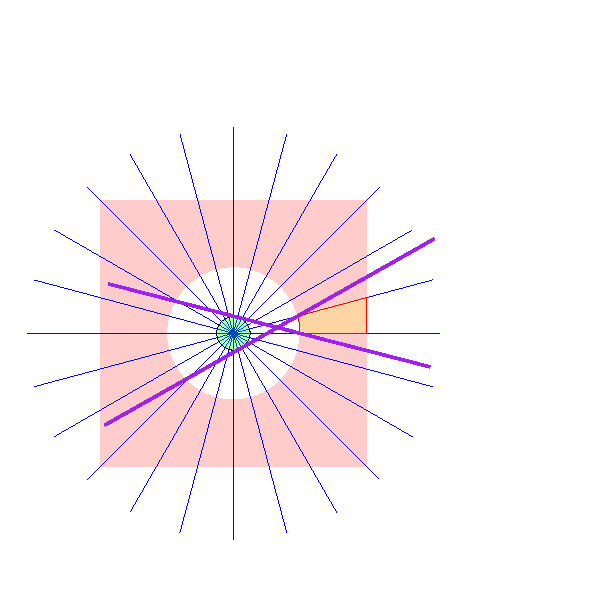
\includegraphics{figs/partition}}
    \caption{}
    \figlab{partition}
\end{figure}


\begin{lemma}
    \lemlab{refine:d:w}%
    %
    Given a $\eps^{-1}$-\SSPD $\WS$ of $n$ points in the plane, one
    can refine it, into a $\eps^{-1}$-\SSPD $\WS'$, such that each
    pair $\Pair = \{ \PSX, \PSY \} \in \WS'$ is contained in a
    $\eps$-double-wedge $\DW_\Pair$, such that $\PSX$ and $\PSY$ are
    contained in the two different faces of the double wedge
    $\DW_\Pair$. We have that $|\WS'| = O(|\WS|/\eps)$ and
    $\WeightX{\WS'} = O(\WeightX{\WS'}/\eps)$. The construction time
    is proportional to the weight of $\WS'$.
\end{lemma}
\begin{proof}
    By using \lemref{chop:easy}, we can assume that $\WS$ is (say)
    $(10/\eps)$-separated.  Now, the algorithm scans the pairs of
    $\WS$. For each pair $\Pair = \{ \PSX, \PSY \} \in \WS$, assume
    that $\diameterX{\PSX} < \diameterX{\PSY}$. Let $\disk$ be the
    smallest axis-parallel square containing $\PSX$, centered at point
    $\cen$.  Partition the plane around $\cen$, by drawing around it
    $O(1/\eps)$ lines with the angle between any two consecutive lines
    being at most (say) $\eps/4$, see \figref{partition}. This
    partition the plane into a set of cones $\ConeSet$. For a cone
    $C \in \ConeSet$, observe that there exists a $\eps$-double-wedge
    that contains $\PSX$ on one side, and $\PSY \cap C$. To see that,
    take the double-wedge formed by the cross tangents between
    $\CHX{\PSX}$ and $\CHX{\PSY \cap C}$, where $\CHX{\PSX}$ denotes
    the convex-hull of $\PSX$.
\end{proof}


% -----------------------------------------------------------------------
\subsubsection{Delaunay triangulation}

We need the following well known property of Delaunay triangulation,
which would play a center role in our construction.

\begin{claim}
    \clmlab{d:t:connected}%
    %
    For a set of points $\PS \subseteq \Re^2$ in general position, let
    $\DT = \DTX{\PS}$ denote its Delaunay triangulation.  Then, for
    any close disk $\disk$, we have $\restrictY{\DTX{\PS}}{\disk}$ is
    connected.
\end{claim}


\begin{proof}
    We first prove that for any (close) disk $\disk$ with two points
    $\pa,\pb\in \PS$ on its boundary, there is a path between $\pa$
    and $\pb$ in $\restrictY{\DT}{\disk}$.  The proof is by induction
    over the number $m$ of points of $\PS$ in the interior of $\disk$:
    \begin{compactitem}
        \item{} $m=0$: The disk $\disk$ contains no points of $\PS$ in
        its interior, and thus $\pa \pb$ is an edge of the Delaunay
        triangulation, as $\disk$ testifies.

        \begin{figure}[h]
            \phantom{}\hfill%
            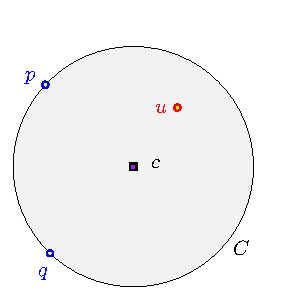
\includegraphics[page=1]{figs/shrink}%
            \hfill%
            \includegraphics[page=2]{figs/shrink}%
            \hfill%
            \includegraphics[page=3]{figs/shrink}%
            \hfill%
            \phantom{}%
            \caption{}
            \figlab{shrink}
        \end{figure}
        \item $m >0$: Let $\pc\in \PS$ be a point in the interior of
        $\disk$. We move the center $\cen$ of $\disk$ in the direction
        of $\pa$, shrinking $\disk$ in the process, so that the radius
        the disk is $\dY{\cen}{\pa}$, until we get a disk
        $\disk' \subseteq \disk$ such that $\pc$ is on the boundary of
        $\disk'$, see \figref{shrink}. Observe that $\pa$ and $\pc$
        are on the boundary of the new disk, and
        $|\interiorX{\disk'} \cap \PS| < |\interiorX{\disk} \cap
        \PS|$. Thus, by induction, there is a path $\gamma'$ between
        $\pa$ and $\pc$ in
        $\restrictY{\DT}{\disk'} \subseteq
        \restrictY{\DT}{\disk}$. Similarly, there must be a path
        $\gamma''$ between $\pc$ and $\pb$, and concatenating the two
        paths results in a path between $\pa$ and $\pb$ in
        $\restrictY{\DT}{\disk}$.
    \end{compactitem}
    \medskip%
    \noindent
    Back to the original claim.  For any two points
    $\pa,\pb \in \disk \cap \PS$ one can get a disk
    $\disk' \subseteq \disk$ that contains $\pa$ and $\pb$ on its
    boundary.  Indeed, shrink the radius of $\disk$ till, say, $\pa$
    is on the boundary, and them move the center of the disk towards
    $\pa$ while shrinking the size of the disk to maintain $\pa$ on
    the boundary, until $\pb$ is also on the boundary of the shrank
    disk.
\end{proof}



%%%%%%%%%%%%%%%%%%%%%%%%%%%%%%%%%%%%%%%%%%%%%%%%%%%%%%%%%%%%%%%%%%%%%%%%%
\subsection{The construction of local spanners for disks}

\subsubsection{The construction}

The input is a set $\PS$ of $n$ points in the plane (in general
position) with $\spread = \spreadX{\PS}$, and a parameter
$\eps \in (0,1)$.

The algorithm computes a $1/\epsA$-\WSPD $\WS$ of $\PS$ using the
algorithm of \lemref{s:s:p:d:spread}, where $\epsA = \eps/6$.  For
each pair $\Pair = \{\PSX, \PSY \} \in \WS$, the algorithm computes
the Delaunay triangulation $\DT_{\Pair} = \DTX{ \PSX \cup \PSY}$. The
algorithm adds all the edges in $\DT_{\Pair} \cap (\PSX \otimes \PSY)$
to the computed graph $\G$.

\subsubsection{Analysis}

\paragraph{Size.}

For each pair $\Pair = \{\PSX, \PSY\}$ in the \WSPD, its Delaunay
triangulation contains at most with $O( |\PSX| + |\PSY|)$ edges. As
such, the number of edges in the resulting graph is bounded by
\begin{equation*}
    \sum_{\{\PSX, \PSY\} \in \WS} O\bigl( |\PSX| + |\PSY| \bigr)
    =%
    O\pth{ \WeightX{\WS} }%
    =%
    O\pth{ \frac{n\log \spread}{{\epsA}^{2}}},
\end{equation*}
by \lemref{s:s:p:d:spread}.


\paragraph{Construction time.}
The construction time is bounded by
\begin{equation*}
    \sum_{\{\PSX, \PSY\} \in \WS} O\bigl( (|\PSX| + |\PSY|) \log
    (|\PSX| + |\PSY|)  \bigr)
    =%
    O\pth{ \WeightX{\WS} \log n }%
    =%
    O\pth{ \frac{n\log \spread \log n}{{\epsA}^{2}}},    
\end{equation*}

\paragraph{Local spanner property.}

\begin{lemma}
    Let $\G$ be the graph constructed above for the point set
    $\PS$. Then, for any (close) disk $\disk$, and any two points
    $\px, \py \in \PS \cap \disk$, we have that
    $\restrictY{\G}{\disk}$ has a $(1+\eps)$-path between $\px$ and
    $\py$. That is, $\G$ is a $(1+\eps)$-local spanner for disks.
\end{lemma}

\begin{proof}
    The proof is by induction on the distance between $\pa$ and $\pb$
    (or more precisely, the rank of their distance among the
    $\binom{n}{2}$ pairwise distances).  Consider the pair
    $\Pair = \{ \PSX, \PSY \}$ such that $\px \in \PSX$ and
    $\py \in \PSY$.

    For the base case, consider the case that $\px$ is the
    nearest-neighbor to $\py$ in $\PS$, and $\py$ is the
    nearest-neighbor to $\px$ in $\PS$.  It must be, because of the
    separation property of $\Pair$, that $\PSX$ and $\PSY$ are
    singletons. Indeed, if $\PSX$ contains another point, then $\py$
    would not be the nearest-neighbor to $\px$ (this is true for
    $\epsA < 0.5$). As such, $\px \py \in \DT_\Pair$,
    $\px, \py \in \disk$, and the edge $\px \py \in \EGX{\G}$,
    implying the claim.

    For the inductive step, observe that , the claim follows if
    $\px \py \in \DT_\Pair$, so assume this is not the case. By the
    connectivity of $\DT_\Pair \cap \disk$, see
    \clmref{d:t:connected}, there must be points
    $\px' \in \PSX \cap \disk$, $\py' \in \PSY \cap \disk$, such that
    $\px'\py' \in \EGX{ \DT_\Pair}$. As such, by construction, we have
    that $\px'\py' \in \EGX{\G}$. Furthermore, by the separation
    property, we have that
    \begin{equation*}
        \max \pth{ \diameterX{\PSX}, \diameterX{\PSY} }%
        \leq%
        \epsA \cdot \dsY{\PSX}{\PSY}%
        \leq%
        \epsA \ell, 
    \end{equation*}
    where $\ell = \dY{\px}{\py}$. In particular,
    $\dY{\px'}{\px} \leq \epsA \ell$ and
    $\dY{\py'}{\py} \leq \epsA \ell$. As such, by induction, we have
    $\dGZ{\G}{\px}{\px'} \leq (1+\eps)\dY{\px}{\px'} \leq
    (1+\eps)\epsA \ell$ and
    $\dGZ{\G}{\py}{\py'} \leq (1+\eps)\dY{\py}{\py'} \leq
    (1+\eps)\epsA \ell$.  Furthermore,
    $\dY{\px'}{\py'} \leq (1+2\epsA)\ell$. As $\px'\py' \in \EGX{\G}$,
    we have
    \begin{align*}
      \dGZ{\G}{\px}{\py}%
      &\leq%
        \dGZ{\G}{\px}{\px'}%
        +\dY{\px'}{\py'}
        +
        \dGZ{\G}{\py'}{\py}%
        \leq%
        (1+\eps)\epsA \ell
        +(1+2\epsA)\ell
        + (1+\eps)\epsA \ell
        \leq%
        \pth{ 2\epsA +1+2\epsA + 2\epsA } \ell        
      \\&%
      =%
      \pth{ 1+ 6\epsA  } \ell        
      \leq%
      \pth{ 1+ \eps  } \dY{\px}{\py},
    \end{align*}
    if $\epsA \leq \eps/6$.
\end{proof}

\paragraph{The result.}

\begin{theorem}
    \thmlab{main:1}%
    %
    Let $\PS$ be a set of $n$ points in the plane, and let
    $\eps \in (0,1)$ be a parameter. The above algorithm constructs a
    local $(1+\eps)$-spanner $\G$ for disks. The spanner has
    $O\pth{ \eps^{-2} n\log \spread }$, with running time
    $O\pth{ \eps^{-2} n\log \spread \log n }$.  Formally, for any disk
    $\disk$ in the plane, and any two points
    $\pa, \pb \in \PS \cap \disk$, we have a $(1+\eps)$-path in
    $\restrictY{\G}{\disk}$.
\end{theorem}

% ------------------------------------------------------------------------
\subsubsection{Applications and comments}


\begin{defn}
    Given a region $R$ in the plane and a point set $\PS$, consider
    two points $\pa, \pb \in \PS$. The edge $\pa \pb$ is \emphw{safe}
    in $R$, if there is a disk $\disk$ such that
    $\pa,\pb \in \disk \subseteq R$. Let $\GY{\PS}{R}$ be the graph
    formed by all the safe edges in $\PS$ for $R$. Note, that his
    graph might have a quadratic number of edges in the worst case.
\end{defn}

Observe that $\GY{\Re^2}{\PS}$ is a clique.

\begin{corollary}
    Let $\PS$ be a set of $n$ points in the plane, and let
    $\eps \in (0,1)$ be a parameter, and let $\G$ be a local
    $(1+\eps)$-spanner for disks. Then, for $R$ be an region in the
    plane, and consider the graph $\GA = \GY{\PS}{R}$. Then
    $\restrictY{\G}{R}$ is a $(1+\eps)$-spanner for
    $\restrictY{\GA}{R}$. Formally, for any two points
    $\pa, \pb \in \PS \cap R$, we have that
    $\dGZ{\GA}{\pa}{\pb} \leq (1+\eps)\dGZ{\G}{\pa}{\pb}$.

    In particular, for any convex region $C$, the graph $\G \gminus C$
    is a $(1+\eps)$-spanner for $\GY{\Re^2}{\PS} \gminus C$.
\end{corollary}
\begin{proof}
    Consider the shortest path $\pi = u_1 u_2 \ldots u_k$ between
    $\pa$ and $\pb$ in $\dGZ{\GA}{\pa}{\pb}$. Every edge
    $e_i = u_i u_{i+1}$ has a disk $\disk_i$ such that
    $u_i, u_{i+1} \in \disk_i \subseteq R$. As such, there is a
    $(1+\eps)$-path between $u_i$ and $u_{i+1}$ in
    $\restrictY{\G}{\disk_i} \subseteq
    \restrictY{\G}{R}$. Concatenating these paths directly yields the
    desired result.

    The second claim follows by observing that the complement of $C$
    is the union of halfspaces, and halfspaces can be considered to be
    ``infinite'' radius disks. As such, the above argument applies
    verbatim.
\end{proof}

\paragraph{But why not \SSPD?}

The result of \thmref{main:1} is somewhat disappointing as it depends
on the spread of the point set (logarithmically, but still). A natural
way is to try and emulate the construction of Abam \etal
\cite{abfg-rftgs-09} and use \SSPD instead of \WSPD. The total weight
of the \SSPD is near linear (with no dependency on the
spread). Furthermore, after some post processing, one can assume every
pair $\Pair = \{ \PSX, \PSY \}$ is angularly $\eps$-separated -- that
is, there is a double wedge with angle $\leq \eps$, such that $\PSX$
and $\PSY$ are of different sides of the double wedge. The problem is
that for the local disk $\disk$, it might be the bridge edge between
$\PSX$ and $\PSY$ that is in $\DT_\Pair \cap \disk$ is much longer
than the two points of interest. This somewhat counter-intuitive
situation is illustrated in \figref{bad}.

\begin{figure}[h]
    \phantom{} \hfill%
    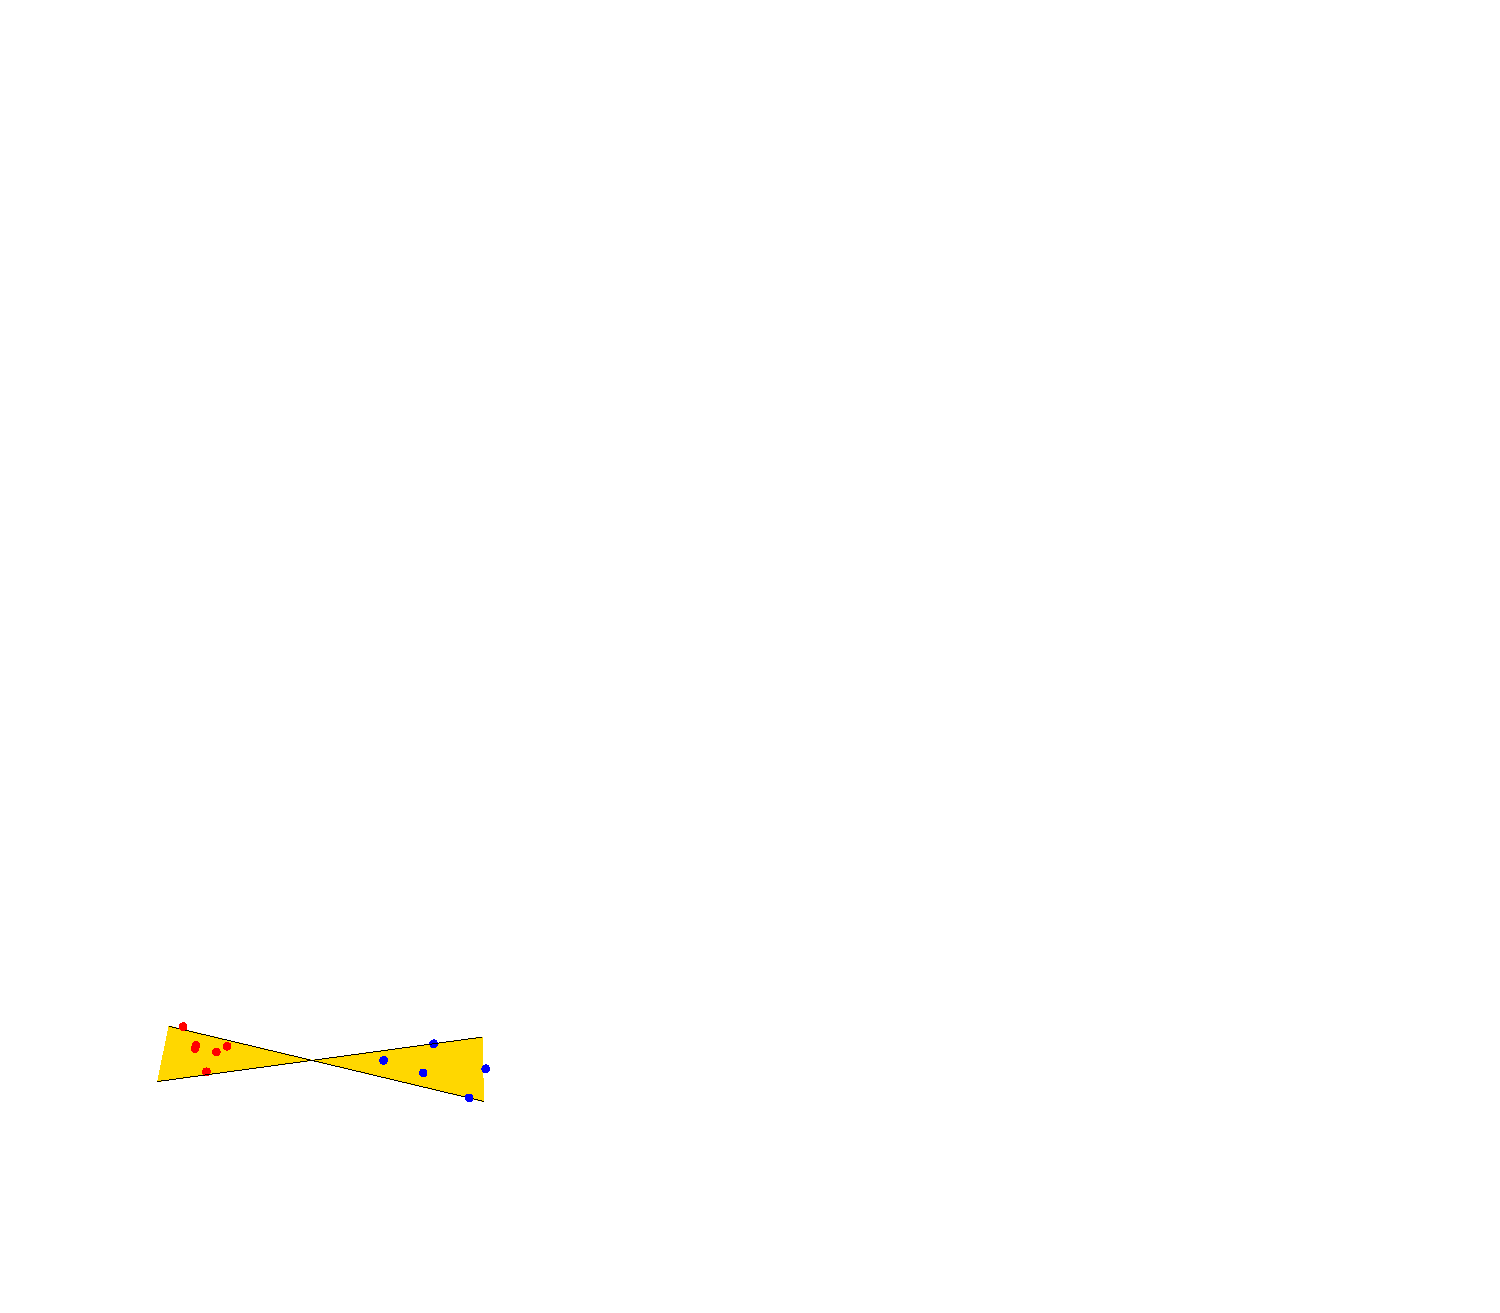
\includegraphics[page=1]{figs/bad_example} \hfill%
    \includegraphics[page=2]{figs/bad_example} \hfill%
    \includegraphics[page=3]{figs/bad_example} \hfill%
    \phantom{}
    \caption{A bridge too far -- the only surviving bridge between the
       red and blue points is too far to be useful if the sets are
       points are not well separated.}
    \figlab{bad}
\end{figure}



%%%%%%%%%%%%%%%%%%%%%%%%%%%%%%%%%%%%%%%%%%%%%%%%%%%%%%%%%%%%%%%%%%%%%%%%%
%%%%%%%%%%%%%%%%%%%%%%%%%%%%%%%%%%%%%%%%%%%%%%%%%%%%%%%%%%%%%%%%%%%%%%%%%
%%%%%%%%%%%%%%%%%%%%%%%%%%%%%%%%%%%%%%%%%%%%%%%%%%%%%%%%%%%%%%%%%%%%%%%%%


\subsection{A local spanner for axis parallel squares}

One can modify the above construction for axis-parallel squares, and
get a local spanner without dependency on the spread.

\subsubsection{Construction}

The input is a point set $\PS$ of $n$ points in the plane, and an
approximation parameter $\eps \in (0,1/2)$.  We assume that the input
point set $\PS$ is in general position. Specifically, no two points of
$\PS$ share a coordinate value, or appear in opposing corners of an
axis-parallel square -- this can be ensured by slightly perturbing the
points if necessary.


One can define the Delaunay triangulation when the unit ball is
replaced by the unit square. Formally, in this triangulation two
points are connected $\iff$ there is a square that contains these two
points on its boundary and no points in its interior. Let
$\DT_\square$ denote the resulting \emphw{$L_\infty$-Delaunay
   triangulation}.

Let $\epsA = \eps/20$.  Instead of constructing a \WSPD, the algorithm
computes a $1/\epsA$-\SSPD $\WS$, using the algorithm of
\thmref{S:S:P:D:main}. Increasing the weight and number of pairs by a
factor of $O(1/\epsA)$, by using the algorithm of \lemref{refine:d:w},
one can assume that every pair $\{ \PSX, \PSY \} \in \WS$ is not only
semi-separated, but also there is an associated double wedge of angle
$\leq \epsA$.  The algorithm now computes the ``square'' Delaunay
triangulation for each such pair, and adds the edges of the
triangulation to the resulting graph $\G$.



\subsubsection{Analysis}

\paragraph{Size and running time.}

Computing the \SSPD takes $O\pth{n \epsA^{-2} \log n}$ time, and the
refinement takes $O\pth{n \epsA^{-3} \log n}$ time (which is also the
weighted of the resulting \SSPD). The number of edges of each
$L_\infty$-Delaunay triangulation for a pair is proportion to its
weight, which implies that the total number of edges in the resulting
graph $\G$ is $O\pth{ \epsA^{-3} n\log n}$. Computing all these
Delaunay triangulations takes $O\pth{ \epsA^{-3}n \log^2 n}$ time.


\paragraph{Shrinking squares.}
We need the following lemma about shrinking of axis-parallel squares.
Observe that this property definitely does not hold for disks, as
illustrated in \figref{bad}.

\begin{lemma}
    \lemlab{shrink:squars}%
    %
    (A) Let $\sqr$ be an axis parallel square in the plane, and let
    $\pa, \pb$ be two arbitrary points in $\sqr$. Then, there is a
    square $\sqrA \subseteq \sqr$ that contains $\pa$ and $\pb$ on its
    boundary.

    (B) Let $\PSX, \PSY$ be two point sets in the plane, such that
    $\PSX' = \PSX \cap \sqr \neq \emptyset$ and
    $\PSY' = \PSY \cap \sqr \neq \emptyset$. Let
    $\px \in \PSX, \py \in \PSY$ be the two points realizing
    $\dsZ{\infty}{\PSX'}{\PSY'} = \min_{\pa \in \PSX', \pb \in \PSY'}
    \dZ{\infty}{\pa}{\pb}$. Then, there is a square
    $\sqrA \subseteq \sqr$ that contains $\px$ and $\py$ on its
    boundary, and $\sqrA$ does not contain any other point of
    $\PSX \cup \PSY$.
\end{lemma}
\begin{proof}
    (A) Start shrinking $\sqr$ around its center till it contains one
    of the points (say $\pa$ is on its boundary. Next, move the center
    of the square towards $\pa$ till the boundary of the continuously
    shrinking square passes through $\pb$. If $\pa$ and $\pb$ lies on
    adjacent edges, then continue the shrinking process by moving the
    center towards the common corner of the shared edges -- this
    process stops when one of the points is on the corner of the
    square.  Clearly, the resulting square $\sqrA$ is the desired
    square, see \figref{shrink:sq}.

    \begin{figure}[h]
        \phantom{}\hfill%
        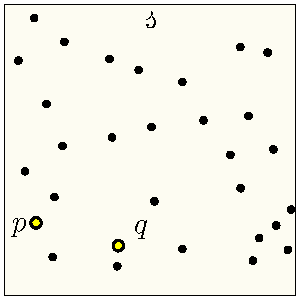
\includegraphics[page=1,width=0.2\linewidth]{figs/shrink_sq}
        \hfill%
        \includegraphics[page=2,width=0.2\linewidth]{figs/shrink_sq}%
        \hfill%
        \includegraphics[page=3,width=0.2\linewidth]{figs/shrink_sq}%
        \hfill%
        \includegraphics[page=4,width=0.2\linewidth]{figs/shrink_sq}
        \hfill\phantom{}%

        \caption{}
        \figlab{shrink:sq}
    \end{figure}

    (B) Let $r = \dsZ{\infty}{\PSX'}{\PSY'}$. By (A), there is a
    square $\sqrA \subseteq \sqr$ having $\px$ and $\py$ on apposing
    sides. As such, the sidelength of $\sqrA$ is $r$. Assume for
    contradiction, that there is some other point
    $\px' \in \PSX \cap \sqrA$. By our general position assumption,
    $\px'$ is in the interior of $\sqrA$, and in particular,
    $\dZ{\infty}{\px'}{\py} < r$, which is a contradiction to the
    choice of $\px$ and $\py$.
\end{proof}

\paragraph{Local spanner property.}
\begin{lemma}
    \lemlab{squares}%
    %
    For any axis parallel square $\sqr$ in the plane, and any two
    points $\pa, \pb \in \PS \cap \sqr$, we have a $(1+\eps)$-path in
    $\restrictY{\G}{\sqr}$.
\end{lemma}
\begin{proof}
    Consider two points $\px, \py \in \PS \cap \sqr$, where $\sqr$ is
    some arbitrary square. There exists a pair
    $\Pair = \{ \PSX, \PSY \} \in \WS$ such that $\px \in \PSX$ and
    $\py \in \PSY$, and this pair is $\epsA^{-1}$-semi separated and
    is also separated by a double wedge of angle $\leq \epsA$.  See
    \figref{infty:spanner}.  Furthermore, assume that
    $\diameterX{\PSX} < \diameterX{\PSY}$.
 
    \begin{figure}[h]
        \hfill%
        {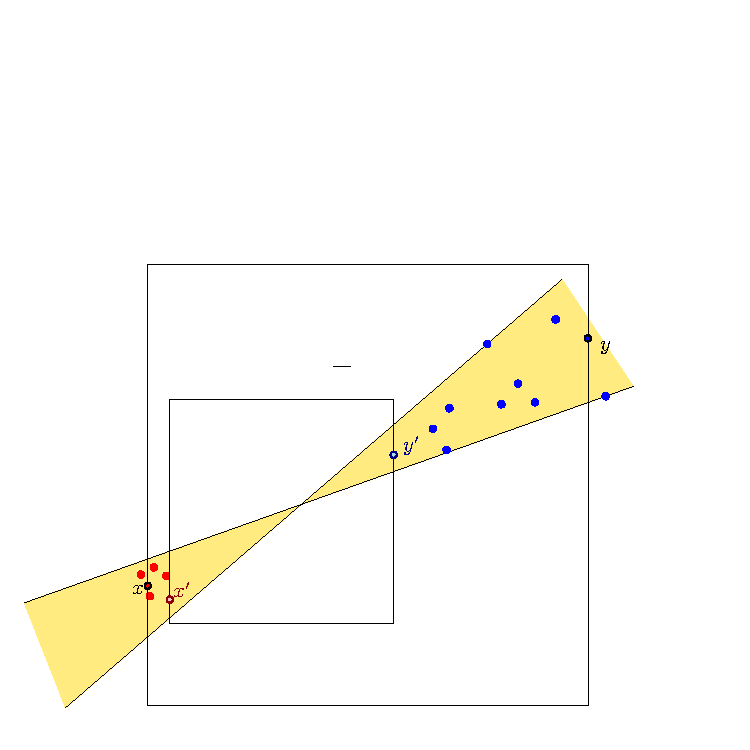
\includegraphics{figs/spanner_sq}} \hfill%
        \phantom{}%
        % 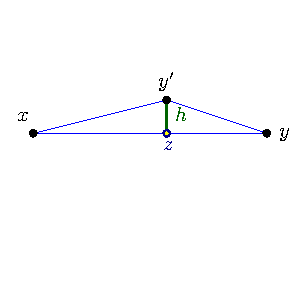
\includegraphics{figs/triangle}%
        \caption{}
        \figlab{infty:spanner}
    \end{figure}

    Let $\PSX' = \PSX \cap \sqr$ and $\PSY' = \PSY \cap \sqr$, and
    consider the two points $\px' \in \PSX'$ and $\py' \in \PSY'$
    realizing $r = \dsZ{\infty}{\PSX'}{\PSY'}$. By
    \lemref{shrink:squars} there exists a square $\sqrA$ containing
    $\px', \py'$ on its boundary (on two apposing edges), such that
    $\sqrA \subseteq \sqr$, and $\sqrA$ contains no other points
    $\PSX \cup \PSY$. By construction, we have that $\px'\py'$ is the
    $L_\infty$-Delaunay triangulation of $\Pair$, and thus
    $\px' \py' \in \G$. Since $\dY{\px}{\px'} \ll \dY{\px}{\py}$, we
    have by induction that
    $\dGZ{\G}{\px}{\px'} \leq (1+\epsA)\dY{\px}{\px'}$.

    % \newpage

    
    Let $\ell = \dY{\px'}{\py'}$. By the semi-separation property and
    since $\diameterX{\PSX} < \diameterX{\PSY}$.  we have that
    \begin{equation*}
        \dY{\px}{\px'}%
        \leq%
        \diameterX{\PSX}%
        \leq%
        \epsA \dGZ{2}{\PSX}{\PSY}%
        =%
        \epsA \sqrt{2} \dGZ{\infty}{\PSX}{\PSY}%
        \leq 
        2
        \epsA \ell.
    \end{equation*}
    Since $\dY{\px}{\px'} \ll \dY{\px}{\py}$, and by induction we have
    that
    \begin{equation*}
        \dGZ{\G}{\px}{\px'}%
        \leq%
        (1+\eps)\dY{\px}{\px'}
        \leq%
        (1+\eps) 2\epsA \ell
        \leq%
        4\epsA \ell.
    \end{equation*}
    By the triangle inequality, we have
    \begin{equation*}
        (1-2\epsA)\ell
        \leq
        \dY{\px'}{\py'} - \dY{\px}{\px'}
        \leq%
        \dY{\px}{\py'}%
        \leq%
        (1+2\epsA)\ell.
    \end{equation*}


    \begin{figure}[h]
        \hfill%
        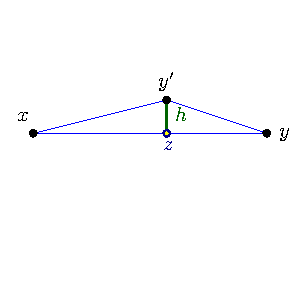
\includegraphics{figs/triangle}%
        \hfill%
        \phantom{}%
        \caption{}
        \figlab{triangle}
    \end{figure}

    Consider the triangle $\triangle \px \py' \py$, and observe that
    by the double-wedge property
    $\alpha = \angle \py' \px \py \leq \epsA$.  Let $\pz$ be the
    projection of $\py'$ to $\px \py$, and let
    \begin{equation*}
        h%
        =%
        \dY{\py'}{ \pz}%
        =%
        \dY{\px}{\py'} \sin \alpha
        \leq
        \dY{\px}{\py'} \sin \epsA
        \leq%
        \dY{\px}{\py'}  \epsA
        \leq%
        \epsA (1+2 \epsA)\ell
        \leq 
        2 \epsA \ell,
    \end{equation*}
    as $\epsA \in (0,1/10)$, the monotonicity of $\sin$ in this range,
    and as $\sin \epsA \leq \epsA$.
    
    We have that
    $\dY{\px}{\pz} \leq \dY{\px}{\py'} \leq
    (1+2\epsA)\ell$. Similarly, we have
    \begin{equation*}
        \dY{\px}{\pz}%
        =%
        \dY{\px}{\py'} \cos \alpha
        \geq%
        (1-\alpha^2/2)\dY{\px}{\py'} 
        \geq 
        (1-\epsA^2/2)(1-2\epsA)\ell
        \geq
        (1-3\epsA)\ell.
    \end{equation*}


    By the triangle inequality, we have that
    \begin{equation*}
        \dY{\py'}{\py}
        \geq%
        \dY{\px}{\py}
        -\dY{\py'}{\px}        
        \geq%
        \dY{\px}{\py}
        - (1+2\epsA)\ell.
    \end{equation*}
    As for an upper bound, we have
    \begin{align*}
      \dY{\py'}{\py}
      &\leq%
        \dY{\pz}{\py} + h%
        \leq%
        \dY{\px}{\py} - \dY{\px}{\pz} +
        2 \epsA \ell
        \leq
        \dY{\px}{\py} - (1-3\epsA)\ell 
        +2 \epsA \ell
      \\&
      = 
      \dY{\px}{\py} - (1-5\epsA)\ell 
      <%
      \dY{\px}{\py}.
    \end{align*}
    As such, by induction
    $\dGZ{\G}{\py'}{\py} \leq (1+\eps) \dY{\py'}{\py}$.

    We thus have that
    \begin{align*}
      \dGZ{\G}{\px}{\py}%
      &\leq%
        \dGZ{\G}{\px}{\px'} + \dY{\px'}{\py'}
        +
        \dGZ{\G}{\py'}{\py}%
        \leq%
        4\epsA \ell
        +
        \ell
        +
        (1+\eps) \dY{\py'}{\py}
      \\&
      \leq%
      (1+4\epsA) \ell
      +
      (1+\eps) \pth{\bigl.
      \dY{\px}{\py} - (1-5\epsA)\ell }
      \\&
      =%
      \bigl[1+4\epsA
      - (1+\eps)(1-5\epsA)\bigr]\ell 
      +
      (1+\eps)
      \dY{\px}{\py}%
      \\&
      \leq%
      (1+\eps)
      \dY{\px}{\py},
    \end{align*}
    for $\epsA \leq \eps/20$, as
    \begin{math}
        1+4\epsA - (1+\eps)(1-5\epsA)%
        \leq%
        1+\eps/5 - (1+\eps)(1-\eps/4)%
        =%
        \eps/5 -(3/4)\eps + \eps^2/4 < 0,
    \end{math}
    as $\eps < 1$.
\end{proof}

\begin{theorem}
    Let $\PS$ be a set of $n$ points in the plane, and let
    $\eps \in (0,1)$ be an approximation parameter. The above
    algorithm computes a local $(1+\eps)$-spanner $\G$ for axis
    parallel squares.  The construction time is
    $O\pth{\eps^{-3} n \log^2 n}$, and the spanner $\G$ has
    $O\pth{\eps^{-3} n \log n}$ edges.
\end{theorem}

\subsection{Result for other norms}

\subsubsection{The rest}

\sariel{FILL IN *all* THE DETAILS -- this is way too hand wavy --
   including refs, etc}

Using the same argument, we can extend the result for the case where
$\LL$ is the set of all scaled and translated copies, homothets, of a
convex shape $\CC$. While the Delaunay triangulation is not well
defined for all convex shapes, the operation of creating edges between
two points $p,q\in P$ such that there exist a homothet of $\CC$ that
contains only $p$ and $q$ and no other point of $\PS$ is always well
defined, and gives us a graph known as the $\CC$-Delaunay graph of
$\PS$, and denoted $\DG_{\CC}(P)$. The above proof applies almost
verbatim for any convex $\CC$, and proves the connectivity of
$\DG_{\CC}(P)$ for any $L\in \LL$.

We need only to define a suitable shrinking operation for convex
region towards a point, which is possible, for example, by
parameterizing the curve defining the region and leaving the desired
point in the same coordinate of the smaller curve. So, we get a
$(1+\eps)-\LL$ local spanner of size $O(\eps^{-3}n\log n)$ in
$O(\eps^{-2}n\log n)$ time.(


%%%%%%%%%%%%%%%%%%%%%%%%%%%%%%%%%%%%%%%%%%%%%%%%%%%%%%%%%%%%%%%%%%%%%%%%%
%%%%%%%%%%%%%%%%%%%%%%%%%%%%%%%%%%%%%%%%%%%%%%%%%%%%%%%%%%%%%%%%%%%%%%%%%
%%%%%%%%%%%%%%%%%%%%%%%%%%%%%%%%%%%%%%%%%%%%%%%%%%%%%%%%%%%%%%%%%%%%%%%%%

\section{Weak local spanners for regions %
   with bounded aspect ratio}

We would like to build local spanners (of subquadratic size) for
axis-parallel rectangles, but as \figref{bad:rectangles} shows, there
is no hope of achieving this. As such, we need to change the
requirement somewhat.

\begin{figure}
    \centerline{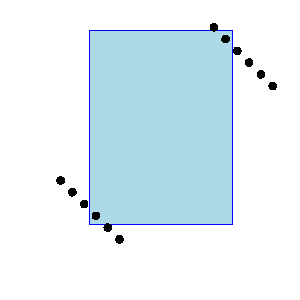
\includegraphics{figs/local_rectangles}}
    \caption{There are quadratic number of pairs of points that has to
       be connected in any local spanner for axis parallel
       rectangles. Indeed, for any point in the top diagonal and
       bottom diagonal, there is an axis parallel rectangle that
       contains only these two points. This holds even if we restrict
       ourselves to fat rectangles of similar size.}
    \figlab{bad:rectangles}
\end{figure}


% \subsection{Shrinking the area of service}

% \subsubsection{Shrinking by the diameter}

One way to shrink a region is as a function of its diameter.

\begin{defn}
    Given a convex region $\body$, let
    \begin{equation*}
        \shrinkDY{\body}{\delta}%
        =%
        \Set{ \pa \in \body }{ \dsY{\pa}{ \Re^2 \setminus \body} \leq \delta
           \diameterX{\body}}.        
    \end{equation*}
    Formally, $\shrinkDY{\body}{\delta}$ is the Minkowski difference
    of $\body$ with a disk of radius $\delta \diameterX{\body}$.
\end{defn}


\begin{defn}
    Consider a (bounded) set $\body$ in the plane. Let $\rinX{\body}$
    be the radius of the largest disk contained inside $\body$.
    Similarly, $\routX{\body}$ is the smallest radius of a disk
    containing $\body$.

    The \emphi{aspect ratio} of a region $\body$ in the plane is
    $\arX{\body} = \routX{\body}/\rinX{\body}$. Given a family $\FF$
    or regions in the plane, its \emphw{aspect ratio} is
    $\arX{\FF} = \max_{\body \in \FF} \arX{\body}$.
\end{defn}

Note, that if a convex region $\body$ has bounded aspect ration, then
$\shrinkDY{\body}{\delta}$ is similar to the result of scaling $\body$
by a factor of $1-O(\delta)$. On the other hand, if $\body$ is long
and skinny, say is has width smaller than
$2 \delta \diameterX{\body}$, then $\shrinkDY{\body}{\delta}$ is
empty.


\begin{lemma}
    Given a family $\FF$ of convex shapes in the plane with
    $\alpha = \arX{\FF}$, a set $\PS$ of $n$ points in the plane, and
    parameters $\delta, \eps \in (0,1)$, let
    $\epsA = \min( \eps, \delta^2)$.  One can construct a graph $\G$
    over $\PS$, in $O(n \epsA^{-1} \log n)$ time, and with
    $O(n/\epsA)$ edges, such that for any $\body \in \FF$, we have
    that for any two points
    $\pa, \pb \in \PS \cap \shrinkDY{\body}{\delta}$ the graph
    $\restrictY{ \body }{\PS}$ has $(1+\eps)$-path between $\pa$ and
    $\pb$.
\end{lemma}

\begin{proof}
    Let $\epsA = \min( \eps, \delta^2)$. Construct, in
    $O(\epsA^{-1} n \log n)$ time, a standard $(1+\epsA)$-spanner $\G$
    for $\PS$ using $O( \epsA^{-1} n)$ edges \cite{ams-dagss-99}.

    So, consider any body $\body \in \FF$, and any two vertex
    $\pa, \pb \in \PS \cap \body'$, where
    $\body'=\shrinkDY{\body}{\delta}$. Let $\ell = \dY{\pa}{\pb}$. Let
    $\pi$ be the shortest path between $\pa$ and $\pb$ in $\G$. Let
    $\Elp$ be the loci of all points $pc$, such that
    $\dY{\pa}{\pc} + \dY{\pc}{\pb} \leq (1+\epsA) \ell$. The region
    $\Elp$ is an ellipse that contains $\pi$. The furthest point from
    the segment $\pa\pb$ in this ellipse is realized by the co-vertex
    of the ellipse. Formally, it is one of the two intersection points
    of the boundary of the ellipse with the line orthogonal to
    $\pa \pb$ that passes through the middle point $\cen$ of this
    segment, see \figref{ellipse}. Let $\pz$ be one of these points.

    \begin{figure}[h]
        \centerline{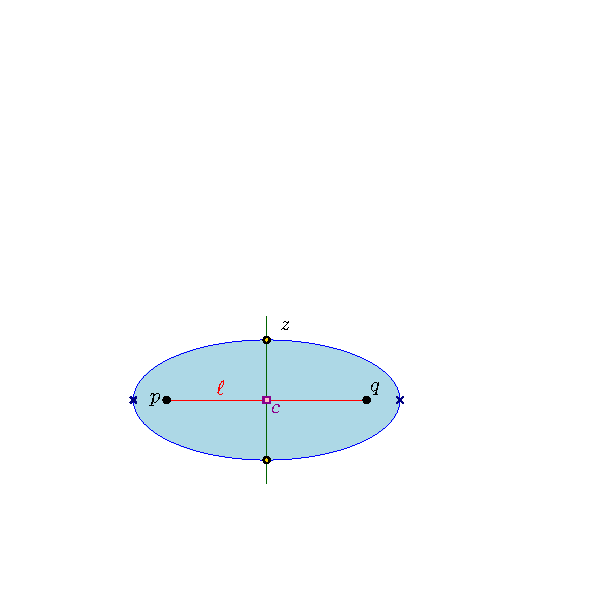
\includegraphics{figs/ellipse}}
        \caption{}
        \figlab{ellipse}
    \end{figure}

    We have that
    \begin{math}
        \dY{\pa}{\pz} = (1+\epsA)\ell/2.
    \end{math}
    Setting $h = \dY{\pz}{\cen}$, we have that
    \begin{equation*}
        h%
        =%
        \sqrt{\dY{\pa}{\pz}^2 - \dY{\pa}{\cen}^2 }
        =%
        \frac{\ell}{2} \sqrt{(1+\epsA)^2 - 1}
        =%
        \frac{\sqrt{\epsA (2+\epsA)}}{2} \ell%
        \leq 
        \sqrt{\epsA} \ell
        \leq 
        \sqrt{\epsA} \diameterX{\body}.
    \end{equation*}
    as $\ell \leq \diameterX{\body'} \leq \diameterX{\body}$.

    For any point $\px \in \body'$, we have that
    $\dsY{\px}{\Re^2 \setminus \body'} \leq \delta \diamX{\body}$.  As
    such, to ensure that $\pi \subseteq \Elp \subseteq \body$, we need
    that
    \begin{math}
        \delta \diamX{\body} \geq h,
    \end{math}
    which holds if
    \begin{math}
        \delta \diamX{\body} \geq \sqrt{\epsA} \diameterX{\body}.
    \end{math}
    This in turn holds if $\epsA \leq \delta^2$. Namely, we have the
    desired properties if $\epsA = \min( \eps, \delta^2)$.
\end{proof}


% Before dwelling into the construction, we start with presenting a
% new pair decomposition that would be useful for our (nefarious)
% purposes, and is of independent interest.

%%%%%%%%%%%%%%%%%%%%%%%%%%%%%%%%%%%%%%%%%%%%%%%%%%%%%%%%%%%%%%%%%%%%%%%%%
%%%%%%%%%%%%%%%%%%%%%%%%%%%%%%%%%%%%%%%%%%%%%%%%%%%%%%%%%%%%%%%%%%%%%%%%%
%%%%%%%%%%%%%%%%%%%%%%%%%%%%%%%%%%%%%%%%%%%%%%%%%%%%%%%%%%%%%%%%%%%%%%%%%

\section{Weak local spanners for axis-parallel rectangles}

\subsection{Quadrant separated pairs decomposition}

For points $\pa = (p_1, \ldots, p_d)$ and $\pb = (q_1, \ldots, q_d)$
in $\Re^d$, let $\pa \prec \pb$ denotes that $\pb$ \emphi{dominates}
$\pa$ coordinate-wise. That is $p_i < q_i$, for all $i$. More
generally, let $\pa <_i \pb$ denote that $\pa_i < \pb_i$. For two
point sets $\PSX, \PSY \subseteq \Re^d$, we use $\PSX <_i \PSY$ to
denote that $\forall \px \in \PSX, \py \in \PSY \quad \px <_i \py$.
In particular $\PSX$ and $\PSY$ are \emphw{$i$-coordinate separated}
if $\PSX <_i \PSY$ or $\PSY <_i \PSX$. A pair $\{ \PSX, \PSY\}$ is
\emphi{quadrant-separated}, if $\PSX$ and $\PSY$ are $i$-coordinate
separated, for $i=1,\ldots, d$.

A \emphi{quadrant-separated pairs decomposition} of a point set
$\PS \subseteq \Re^d$, is a pairs decomposition (see
\defref{pair:decomposition}
$\WS = \bigl\{ \{ \PSX_1, \PSY_1 \}, \ldots, \{ \PSX_s, \PSY_s \}
\bigr\}$ of $\PS$, such that $\{ \PSX_i, \PSY_i\}$ are
quadrant-separated for all $i$.


\begin{lemma}
    \lemlab{d:1}%
    %
    Given a set $\PS$ of $n$ points in $\Re$, one can compute, in
    $O( n \log n)$ time, a \QSPD of $\PS$ with $O(n)$ pairs, and of
    total weight $O( n \log n)$.
\end{lemma}
\begin{proof}
    If $\PS$ is a singleton then there is nothing to do. If
    $\PS = \{ \pa, \pb \}$, then the decomposition is the pair formed
    by the two singleton points.

    Otherwise, let $x$ be the median of $\PS$, such that
    $\PS_{\leq x} = \Set{ \pa \in \PS }{\pa \leq x}$ contains exactly
    $\ceil{n/2}$ points, and $\PS_{> x} = \PS \setminus \PS_{\leq x}$
    contains $\floor{n/2}$ points. Construct the pair
    $\Pair = \{ \PS_{\leq x}, \PS_{> x} \}$, and compute recursively a
    \QSPD{}s $\QS_{\leq x}$ and $\QS_{> x}$ for $\PS_{\leq x}$ and
    $\PS_{> x}$, respectively. The desired \QSPD is
    \begin{math}
        \QS_{\leq x} \cup \QS_{> x} \cup \{ \Pair \}.
    \end{math}
    The bounds on the size and weight of the desired \QSPD are
    immediate.
\end{proof}


\begin{lemma}
    Given a set $\PS$ of $n$ points in $\Re^d$, one can compute, in
    $O( n \log^d n)$ time, a \QSPD of $\PS$ with $O(n \log^{d-1} n)$
    pairs, and of total weight $O( n \log^d n)$.
\end{lemma}
\begin{proof}
    The construction algorithm is recursive on the dimensions, using
    the algorithm of \lemref{d:1} in one dimension.

    The algorithm computes a value $\alpha_d$ that partition the
    values of the points in $d$\th coordinate roughly equally (and is
    distinct from all of them), and let $h$ be a hyperplane parallel
    to the first $d-1$ coordinate axes, and having value $\alpha_d$ in
    the $d$\th coordinate.

    Let $\PS_{\uparrow}$ and $\PS_{\downarrow}$ be the subset of
    points of $\PS$ that are above and below $h$, respectively.  The
    algorithm computes recursively \QSPD{}s $\QS_\uparrow$ and
    $\QSdown$ for $\PSup$ and $\PS_{\downarrow}$, respectively.  Next,
    the algorithm projects the points of $\PS$ to $h$, and let $\PS'$
    be the resulting $d-1$ dimensional point set (after we ignore the
    $d$\th coordinate). Compute recursively a \QSPD $\QS'$ for $\PS'$.

    
    For a point set $\PSX' \subseteq \PS'$, let $\liftX{\PSX'}$ be the
    subset of points of $\PS$ that its projection to $h$ is $\PSX'$.
    The algorithm now computes the set of pairs
    \begin{equation*}
        \widehat{\QS}%
        =%
        \Set{\Bigl.
           \{ \liftX{ \PSX'} \cap \PSup , \liftX{ \PSY' } \cap \PSdown
           \}, \,\,
           \{ \liftX{ \PSX'} \cap \PSdown , \liftX{ \PSY' } \cap \PSup
           \}
        }%
        { \{ \PSX', \PSY' \} \in \QS'}     .
    \end{equation*}
    The desired \QSPD is $\widehat{\QS} \cup \QSup \cup \QSdown$.

    To observe that this is indeed a \QSPD, observe that all the pairs
    in $\QSup, \QSdown$ are quadrant separated by induction. As for
    pairs in $\widehat{\QS}$, they are quadrant separated in the first
    $d-1$ coordinates by induction on the dimension, and separated in
    the $d$ coordinate since one side of the pair comes from $\PSup$,
    and the other side from $\PSdown$.

    As for coverage, consider any pair of points $\pa, \pb \in \PS$,
    and observe that the claim holds by induction if they are both in
    $\PSup$ or $\PSdown$. As such, assume that $\pa \in \PSup$ and
    $\pb \ni \PSdown$. But then there is a pair
    $\{\PSX', \PSY'\} \in \QS'$ that separates the two projected
    points in $h$, and clearly one of the two lifted pairs that
    corresponds to this pair quadrant-separates $\pa$ and $\pb$ as
    desired.

    The number pairs in the decomposition is
    \begin{math}
        N(n,d) = 2N(n,d-1) + 2N\pth{ n/2, d }
    \end{math}
    with $N(n,1) = O(n)$. The solution to this recurrence is
    $N(n,d) = O( n \log^{d-1} n)$.  The total weight of the
    decomposition is
    \begin{math}
        W(n,d) = 2W(n,d-1) + 2W\pth{ n/2, d }
    \end{math}
    with $W(n,1) = O(n \log n)$. The solution to this recurrence is
    $W(n,d) = O( n \log^{d} n)$. Clearly, this also bounds the
    construction time.
\end{proof}

%%%%%%%%%%%%%%%%%%%%%%%%%%%%%%%%%%%%%%%%%%%%%%%%%%%%%%%%%%%%%%%%%%%%%%

\subsection{Weak local spanner for axis parallel rectangles}

For a parameter $\delta \in (0,1)$, and an interval $I = [b,c]$, let
$(1-\delta)I = [t - (1-\delta)r, t+ (1-\delta)r]$ be the shrinking of
$I$ by a factor of $1-\delta$, where $t = (b+c)/2$, and $r = c-b$.


Let $\Rects$ be the set of all axis parallel rectangles in the
plane. For a rectangle $\rect \in \Rects$, with $\rect = I \times J$,
let $(1-\delta)\rect = (1-\delta)I \times (1-\delta)J$ denote the
rectangle resulting from shrinking $\rect$ by a factor of $1-\delta$.

\begin{defn}
    Given a set $\PS$ of $n$ points in the plane, and parameters
    $\eps, \delta \in (0,1)$, a graph $\G$ is a
    \emphw{$(1-\delta)$-local $(1+\eps)$-spanner} for rectangles, if
    for any axis-parallel rectangle $\rect$, we have that
    $\restrictY{\G}{\rect}$ is a $(1+\eps)$-spanner for all the points
    in $(1-\delta)\rect \cap \PS$.
\end{defn}

Observe that rectangles in $\Rects$ might be quite ``skinny'', so the
previous notion of shrinkage used before are not useful in this case.

\subsubsection{Construction for a single quadrant separated pair}
\seclab{pair:edges}

\begin{figure}[t]
    \centering%
    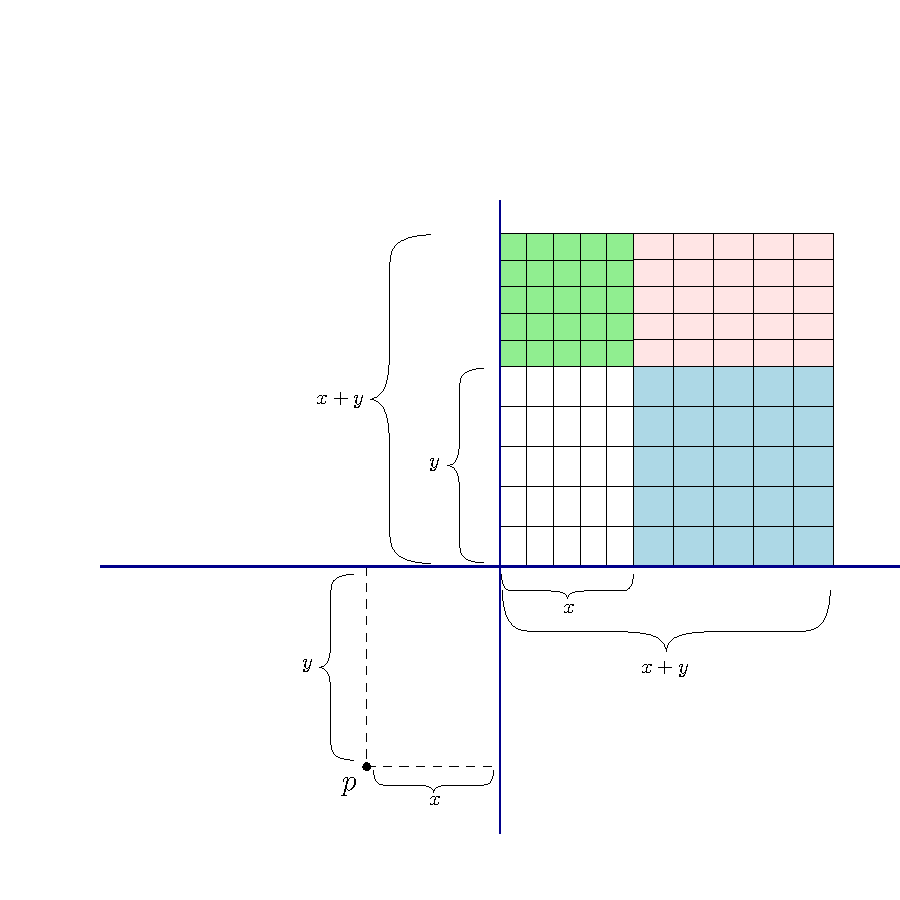
\includegraphics{figs/grid_construction}%
    \caption{The construction of the grid $\grid(\pa,\Pair)$ for a
       point $\pa=(x,y)$ and a pair $\Pair$. We are not showing the
       subrectangles of $\rectA_\nearrow$ as they are not being used
       in the construction.  }
    \figlab{grid}%
\end{figure}

Consider a pair $\Pair = \{\PSX, \PSY \}$ in a \QSPD of $\PS$. The set
$\PSX$ is quadrant-separated from $\PSY$. That is, there is a point
$\cen_\Pair$, such that $\PSX$ and $\PSY$ are contained in two
opposing quadrants in the partition of the plane formed by the
vertical and horizontal line through $\cen_\Pair$.

For simplicity of exposition, assume that $\cen_\Pair = (0,0)$, and
$\PSX \prec (0,0 ) \prec \PSY$. That is, the points of $\PSX$ are in
the negative quadrant, and the points of $\PSY$ are in the positive
quadrant.

Consider a point $\pa \in \PSX$. Its \emphw{set of clients} in $\PSY$,
is
\begin{equation*}
    \clientsY{\pa}{\PSY}%
    =%
    \Set{ \pb \in \PSY }{ \dZ{1}{\pb}{\cen_\Pair}  \leq
       \dZ{1}{\pa}{\cen_\Pair}}.
\end{equation*}

We construct a non-uniform grid $\grid(\pa, \Pair)$ in the square
$[0,x+y]^2$.  To this end, we first partition it into four
subrectangles
\begin{equation*}
    \begin{array}{l|l}
      \rectA_\nwarrow = [0,x] \times [y,x+y]
      &
        \rectA_\nearrow = [x,x+y] \times [y,x+y]\Bigr.\\
      \hline
      \rectA_{\swarrow} = [0,x]\times [0,y]
      &
        \rectA_\searrow = [x,x+y] \times [0,y].\Bigr.\\
    \end{array}
\end{equation*}
Let $\tau > 0$ be an integer number of specified shortly.  We
subpartition each of these rectangles into a $\tau \times \tau$ grid,
where each cell is a scaled $1/\tau$ copy of itself.  See
\figref{grid}. This grid has $O(\tau^2)$ cells. For a cell $\cell$ in
this grid, let $\PSY \cap \cell$ be the points of $\PSY$ contained in
it. We connect $\pa$ to the left-most and bottom-most points in
$\PSY \cap \cell$. This process generates two edges in the constructed
graph for each grid cell, and $O( \tau^2)$ edges overall.

The algorithm repeats this construction for all the points
$\pa \in \PSX$. It does the symmetric construction for all the points
of $\PSY$.


\subsubsection{The construction algorithm}

The algorithm computes a $1/\epsA$-\QSPD $\WS$ of $\PS$, for a
parameter $\epsA$ to be specified shortly. For each pair
$\Pair \in \WS$, the algorithm generates edges for $\Pair$ using the
algorithm of \secref{pair:edges} and adds them to the generated
spanner $\G$.





\subsubsection{Correctness}

\begin{figure}[h]
    \includegraphics[page=2]{figs/grid_2}%
    \hfill%
    \includegraphics[page=3]{figs/grid_2}%
    \hfill%
    \includegraphics[page=4]{figs/grid_2}
    \caption{}
    \figlab{grid:2}
\end{figure}
\begin{lemma}
    Consider a pair $\Pair = \{\PSX, \PSY \}$ in the above
    construction, and a point $\pa =(x,y) \in \PSX$, and its
    associated grid $\grid = \grid(\pa, \Pair)$, where $x \geq
    y$. Consider any axis parallel rectangle $\rect$, such that
    $\pa \in (1-\delta)\rect = I\times J$, and $(1-\delta)\rect$
    intersects a cell $\cell \in \grid$. We have that:
    \begin{compactenumI}
        \item If $\cell \subseteq (1-\delta)\rect$ then
        $(1-\delta)^{-1} \cell \subseteq \rect$.

        \item If $x \geq y$ and
        $\cell \subseteq \rect_\swarrow \cup \rect_\searrow$ then
        $(1-\delta)^{-1} \cell \subseteq \rect$.

        \item If $x \leq y$ and
        $\cell \subseteq \rect_\swarrow \cup \rect_\nwarrow$ then
        $(1-\delta)^{-1} \cell \subseteq \rect$.

        \item If $x \geq y$ and $\cell \subseteq \rect_\nwarrow$, then
        $(1-\delta)^{-1} \bigl(\cell \cap ([-\infty,+\infty]\times
        J)\bigr) \subseteq \rect$.



        \item $\diameterX{\cell} \leq \eps \dsY{\pa}{\cell}$.
    \end{compactenumI}
\end{lemma}
\begin{proof}
    Let $\pa = (\pa_x, \pa_y)$. By construction, the width of $\rect$
    is at least $\pa_x$ and its height is at least $\pa_y$.  $\cell$
\end{proof}

XXXXXXXXXXXXXXXXXxx

\begin{lemma}
    For any axis-parallel rectangle $\rect$, and any two points
    $\pa, \pb \in (1-\delta)\rect \cap \PS$, there exists a
    $(1+\eps)$-path between $\pa$ and $\pb$ in $\G$.
\end{lemma}
\begin{proof}
    ~
\end{proof}



%%%%%%%%%%%%%%%%%%%%%%%%%%%%%%%%%%%%%%%%%%%%%%%%%%%%%%%%%%%%%%%%%%%%%%%%
%%%%%%%%%%%%%%%%%%%%%%%%%%%%%%%%%%%%%%%%%%%%%%%%%%%%%%%%%%%%%%%%%%%%%%%%



We first describe a subroutine for connecting two sets of points, $A$
and $B$, where $A$ is contained in $Q^-$, the negative quadrant of the
plane (i.e., have a negative value $x$-coordinate and a negative value
$y$-coordinate), and $B$ is contained in $Q^+$, the positive quadrant
of the plane.

Our algorithm will connect every point in $A$ to
$O\left(\frac{1}{\eps^2}\right)$ points in the positive quadrant, and
after performing the same process for the points of the symmetrically
defined $B'$, we will have that every rectangle that truly contains
points from $A$ and $B$ will have an edge $(a,b)$ with $a\in A$ and
$b\in B$.

For every point $a = (x',y') \in A$ we define partition the positive
quadrant into $O\left(\frac{1}{\eps^2}\right)$ sets. We consider the
following $\frac{1}{\eps}$ horizontal stripes -
$\forall j\in \{1,...,\frac{1}{\eps}\}$:

\hrule

If $\log_{1+\eps}(1-\eps)<-1$, then there must be an integer $i$ with
the required properties. We now notice that
$(1+\eps)^{-1}=\frac{1}{1+\eps}>(1-\eps)$ [since
$1>(1-\eps)(1+\eps)=(1-\eps^2)$], and so $i$ exists.

The size of the spanner is $\log_{1+\eps}(\alpha)$ times the number of
edges in a convex local spanner, and since
$\log_{1+\eps}(\alpha)=O\left(\frac{\log(\alpha)}{\eps}\right)$, we
have a spanner of size
$O\left(\frac{\log(\alpha)}{\eps (t-1)^{-3}}n\log n\right)$


\subsection{Arbitrary rectangles}

Let $P\subseteq \Re^2$. We first describe a subroutine for connecting
two sets of points, $A$ and $B$, where $A$ is contained in $Q^-$, the
negative quadrant of the plane (i.e., have a negative value
$x$-coordinate and a negative value $y$-coordinate), and $B$ is
contained in $Q^+$, the positive quadrant of the plane.

Our algorithm will connect every point in $A$ to
$O\left(\frac{1}{\eps^2}\right)$ points in the positive quadrant, and
after performing the same process for the points of the symmetrically
defined $B'$, we will have that every rectangle that truly contains
points from $A$ and $B$ will have an edge $(a,b)$ with $a\in A$ and
$b\in B$.

For every point $a = (x',y') \in A$ we define partition the positive
quadrant into $O\left(\frac{1}{\eps^2}\right)$ sets. We consider the
following $\frac{1}{\eps}$ horizontal stripes -
$\forall j\in \{1,...,\frac{1}{\eps}\}$:

\hrule

\begin{equation}
    H_{j}:=\{(x,y)~|~  0 \leq x \leq x'+y'  ,~ (j-1)\cdot \eps y' < y
    \leq j\cdot \eps y'\}
\end{equation}

On top of these we add similarly built vertical stripes:

\begin{equation}
    V_{i}:=\{(x,y)~|~ (j-1)\cdot \eps x' < x \leq j\cdot \eps x',~ 0
    \leq y \leq x'+y' \}
\end{equation}

\hrule

These stripes create a grid which partitions the rectangle $r$ whose
opposite corners are $(0,0)$ and $(|x'|,|y'|)$ into $\frac{1}{\eps^2}$
cells of width $\eps x$ and height $\eps y$. Formally:

\begin{equation}
    C_{i,j}:=\{(x',y')~|~  (i-1)\cdot \eps x < x' \leq i\cdot \eps x,~
    (j-1)\cdot \eps y< y' \leq j\cdot \eps y\}
\end{equation}

We now divide the parts of the stripes that lie outside of the
rectangle $r$. The horizontal stripes are divided into cells of width
$\eps(x+y)$ and height $\eps y$, and the vertical stripes are divided
into cells of width $\eps y$and height $\eps(x+y)$. The extremal cell
in each stripe may be smaller if $x$ or $y$ are not divisible by
$\eps(x+y)$. Formally:

\hrule

These stripes create a grid which partitions the rectangle $r$ whose
opposite corners are $(0,0)$ and $(|x'|,|y'|)$ into $\frac{1}{\eps^2}$
cells of width $\eps x$ and height $\eps y$. Formally:

\begin{equation}
    C_{i,j}:=\{(x',y')~|~  (i-1)\cdot \eps x < x' \leq i\cdot \eps x,~
    (j-1)\cdot \eps y< y' \leq j\cdot \eps y\}
\end{equation}

We now divide the parts of the stripes that lie outside of the
rectangle $r$. The horizontal stripes are divided into cells of width
$\eps(x+y)$ and height $\eps y$, and the vertical stripes are divided
into cells of width $\eps y$and height $\eps(x+y)$. The extremal cell
in each stripe may be smaller if $x$ or $y$ are not divisible by
$\eps(x+y)$. Formally:

\hrule

\begin{equation}
    C_{H_{i,j}}:=\{(x',y')~|~  x' + (i-1)\cdot \eps (x+y) < x' \leq x'
    + i\cdot \eps (x+y),~ (j-1)\cdot \eps y< y' \leq j\cdot \eps y\}
\end{equation}

\begin{equation}
    C_{V_{i,j}}:=\{(x',y')~|~  (i-1)\cdot \eps x < x' \leq i\cdot \eps
    x,~ y + (j-1)\cdot \eps (x+y)< y' \leq y + j\cdot \eps (x+y)\}
\end{equation}

\hrule

The entire construction can be seen in \figref{grid_construction}.


\begin{claim}
    For every rectangle $r\in \LL$ and a pair $(A,B)$ of the SSPD
    s.t. $r_{1-\eps}\cap A \neq \emptyset$ and
    $r_{1-\eps}\cap B \neq \emptyset$, there are two points
    $a\in A, b\in B$ connected by an edge.
\end{claim}

\begin{proof}
    Let $A'=A\cap r_{1-\eps}, B'=B \cap r_{1-\eps}$, and let
    $p= \underset{p'}{argmax}\{||p'||_{\infty}~:~ p'\in A\cup B\}$,
    and assume w.l.o.g that $p\in A'$ and prove that there exist a
    point $q\in B'$ connected to $p$ by an edge.
    
    We take a point $q'\in B'$. Due to the choice of $p$ we have that
    one of the coordinates of $q'$ has a smaller absolute value than
    the same respective coordinate of $p$, and assume w.l.o.g that it
    is the $x$-coordinate. Now, since $\bigcup C_{i,j} \bigcup V_i$
    cover the entire part of $Q^+$ with an absolute $x$ value lower
    that that of $p$, we have that either there is an edge $\{p,q\}$
    in the graph, or there is another point $q$ in the same cell as
    $q'$. Regardless, since the cells are of width $\eps\cdot p.x$ and
    height $\eps\cdot p.y$ ,and $r$ is of width at least $p.x$ and
    height at least $p.y$, we get that the entire cell is inside $r$,
    and therefore there exists an edge as described in the claim.
    
    \hrule

    The entire construction can be seen in
    Figure~\ref{fig:grid_construction}. We can now describe the
    construction of our spanner. For $P\subseteq \Re^2$ we create a
    \QSPD of $P$, and for every pair $(A,B)$ we add an edge between
    every point $a\in A$ (and later reverse the rolls inside the pair)
    to an arbitrary point of $P$ in every cell $C_{i,j}$, to the
    leftmost point of $P$ in every $C_{H_{i,j}}$, and to the
    bottom-most point of $P$ in every $C_{V_{i,j}}$.
\end{proof}

We now prove a lemma that summarizes the properties of the resulted
graph, and which we will then use to prove that our construction
produces an $(\LL, eps)$- local $t$-spanner for the family of
arbitrary axis parallel rectangles.


\begin{claim}
    \label{clm:span_properties}
    For any two points $a,b\in P$ that are properly contained in an
    axis parallel rectangle $r$ ,and are not connected by an edge,
    there exists a point $b'\in r$ such that if w.l.o.g
    $||b-b'|| \leq ||a-c||$ then:
    \begin{enumerate}
        \item $||b-b'|| \leq 3\eps ||a-b||)$, and
        \item there is an edge between $a$ and $b'$.
    \end{enumerate}
    Additionally, the two closest points $p,q\in P$ are connected by
    an edge.
	
\end{claim}

\begin{proof}
    Let $(A,B)$ be the unique pair of the \QSPD such that w.l.o.g
    $a\in A$ and $b\in B$, $A\subseteq Q^-$, $B\subseteq Q^+$, and
    $||b||_{1} \leq ||a||_{1}$. We denote the absolute value of the
    coordinates of a point $p$ by $p.x$ and $p.y$ for the $x$ and $y$
    coordinates respectively. If $b.x \leq a.x$ and $b.y \leq a.y$,
    then by the construction, $a$ is connected to a point $b'$ in the
    cell $C_{i,j}$ containing $b$. Since the cell's dimensions are
    $\eps\cdot a.x \times \eps a.y$, we have that
    $C_{i,j}\subseteq r$, and also:
	
	\begin{equation}
            ||b-b'||\leq \sqrt{(\eps\cdot a.x)^2+(\eps\cdot
               a.y)^2}=\eps\sqrt{a.x^2+a.y^2}\leq \eps(a.x+a.y) \leq
            2\eps||a-b||
        \end{equation}
	
	regardless of the choice of $b'$, as
        $||a-b||\geq||a-(0,0)||\geq \frac{a.x+a.y}{2}$.
	
	If w.l.o.g $a.x\leq b.x$, then since $||b||_{1} \leq
        ||a||_{1}$ we know that $b.y \leq a.y$ meaning that $b$ is
        contained in some cell $C_{H_{i,j}}$. Again, due to the
        dimensions of $C_{H_{i,j}}$ (which are
        $\eps\cdot a.y \time \eps\cdot(a.x+a.y)$) we have that $b'$,
        the leftmost point of $P$ in $C_{H_{i,j}}$, is contained in
        $r$, and also:
	
	\begin{equation}
            ||b-b'||\leq \sqrt{(\eps (a.x+a.y))^2+(\eps\cdot
               a.y)^2}\leq \sqrt{2(\eps (a.x+a.y))^2}
        \end{equation}
	\begin{equation}
            =\sqrt{2}\eps(a.x+a.y) \leq \sqrt{8}\eps||a-b||.
        \end{equation}
	
	In order to prove the second property we only need to notice
        that if w.l.o.g $p\in Q^-$, $q\in Q^+$, and
        $||q||_1\leq ||p||_1$, we have that due to the dimensions of
        the cells we can see by similar calculations that for any
        $\eps\leq \frac{1}{\sqrt{8}}$ we have that $q$ is the only
        point in its cell of the construction, since otherwise we get
        a point $q'$ such that $||q-q'||\leq ||p-q||$.
	
    \end{proof}

    We are left with proving that for a suitable choice of parameters,
    this construction results in a $(\LL,\eps)$ local $t$-spanner.


    % TO DO: this can probably be done faster than the naive way.
    \begin{claim}
	It is possible to construct a $(\LL, \epsA)$ local
        $(1+\epsA')$-spanner of size
        $O\left(\frac{1}{\min\{\eps, \epsA\}}n\log^2n\right)$ in
        $O_d\left(\frac{1}{\eps^2}n\log^{O(d)}n\right)$ time.
    \end{claim}

\begin{proof} 
    Let $\eps = \alpha \min \{\epsA,\epsA'\}$ for some
    $\alpha \leq \frac{1}{12}$. We build a spanner using $\eps$ as the
    parameter for the edge construction process. Due to the choice of
    $\eps$ we have that all of the properties proven in
    Claim~\ref{clm:span_properties} are apply. Also, since we have
    reduced the parameter $\eps$ by a factor of $\frac{1}{2}$ on top
    of the $\frac{1}{3}$ required to get $||b-b'||\leq \eps ||b-a||$,
    we have that there exists a rectangle $r'\subseteq r$ such that
    $b,b'\in_{\eps}r'$. This means that we can recurse on pairs of
    points by their rank (in the set of pairs ordered by distance). In
    the base case we know from Claim~\ref{clm:span_properties} the
    points are connected by an edge, and for the recursion step we get
    that for two points $p,q\in P$ and a rectangle $r$ such that
    $p,q\in_{\eps} r$ we have a point $q'\in P$ such that:
    \begin{enumerate}
        \item $||q-q'||\leq \eps||p-q||$,
        \item there is an edge between $p$ and $q'$, and
        \item there exists a $1+\eps$ spanning path between $q$ and
        $q'$
    \end{enumerate}

    This gives us a path $p\rightarrow q' \rightarrow q$ of length at
    most
	
	\begin{equation}
            ||p-q'||+(1+\eps)||q-q'||\leq
            ||p-q||+(1+\eps)\eps||p-q||\leq (1+\epsA')||p-q||.
        \end{equation}
	
	where the last transition is due to another factor of
        $\frac{1}{2}$ that was incorporated in $\alpha$.
	
	The number of edges is bounded by the size of the \QSPD
        multiplied by $\frac{1}{\eps^2}$, since every occurrence of a
        point in the \QSPD gives rise to
        $O\left(\frac{1}{\eps^2}\right)$ edges by construction.
	
	The runtime of the algorithm is composed of constructing a
        $d$-dimensional orthogonal range tree in time
        $O(n\log^{d-1}n)$, and querying
        $O\left(\frac{1}{\eps^2}\right)$ $d$-dimensional boxes for
        every point in the \QSPD, each in time $O(\log^{d-1}n)$. Since
        the points in the orthogonal range tree are sorted by
        dimension, getting the leftmost or bottom-most point for some
        queries does not affect the runtime.
	
\end{proof}
\hrule


\subsection{Bounded aspect ratio triangles}

The aspect ratio of a triangle is defined as the length of its longest
edge divided by its height as it is measured from that edge. Let $\LL$
be the set of all triangles with aspect ratio at most $\alpha$ for
some $1 < \alpha$. We define a set of slopes, and for each subset of 3
slopes we run the convex region algorithm with $\LL$ as homothets of a
triangle with edges of the 3 chosen slopes. As long as the fixed
angular interval is smaller than
$\epsA = \arctan\left(\frac{\eps/2}{\alpha(1-\eps/2)}\right)$ (see
\figref{triangle_with_shadow}).

This construction creates $\frac{1}{\epsA}$ different convex local
spanners, and so we get a $(1+\eps)$-local spanner for triangles with
bounded aspect ratio in
$O\left(\frac{1}{\epsA^3\eps^3} n\log n\right)$.


\begin{figure}
    \centering
    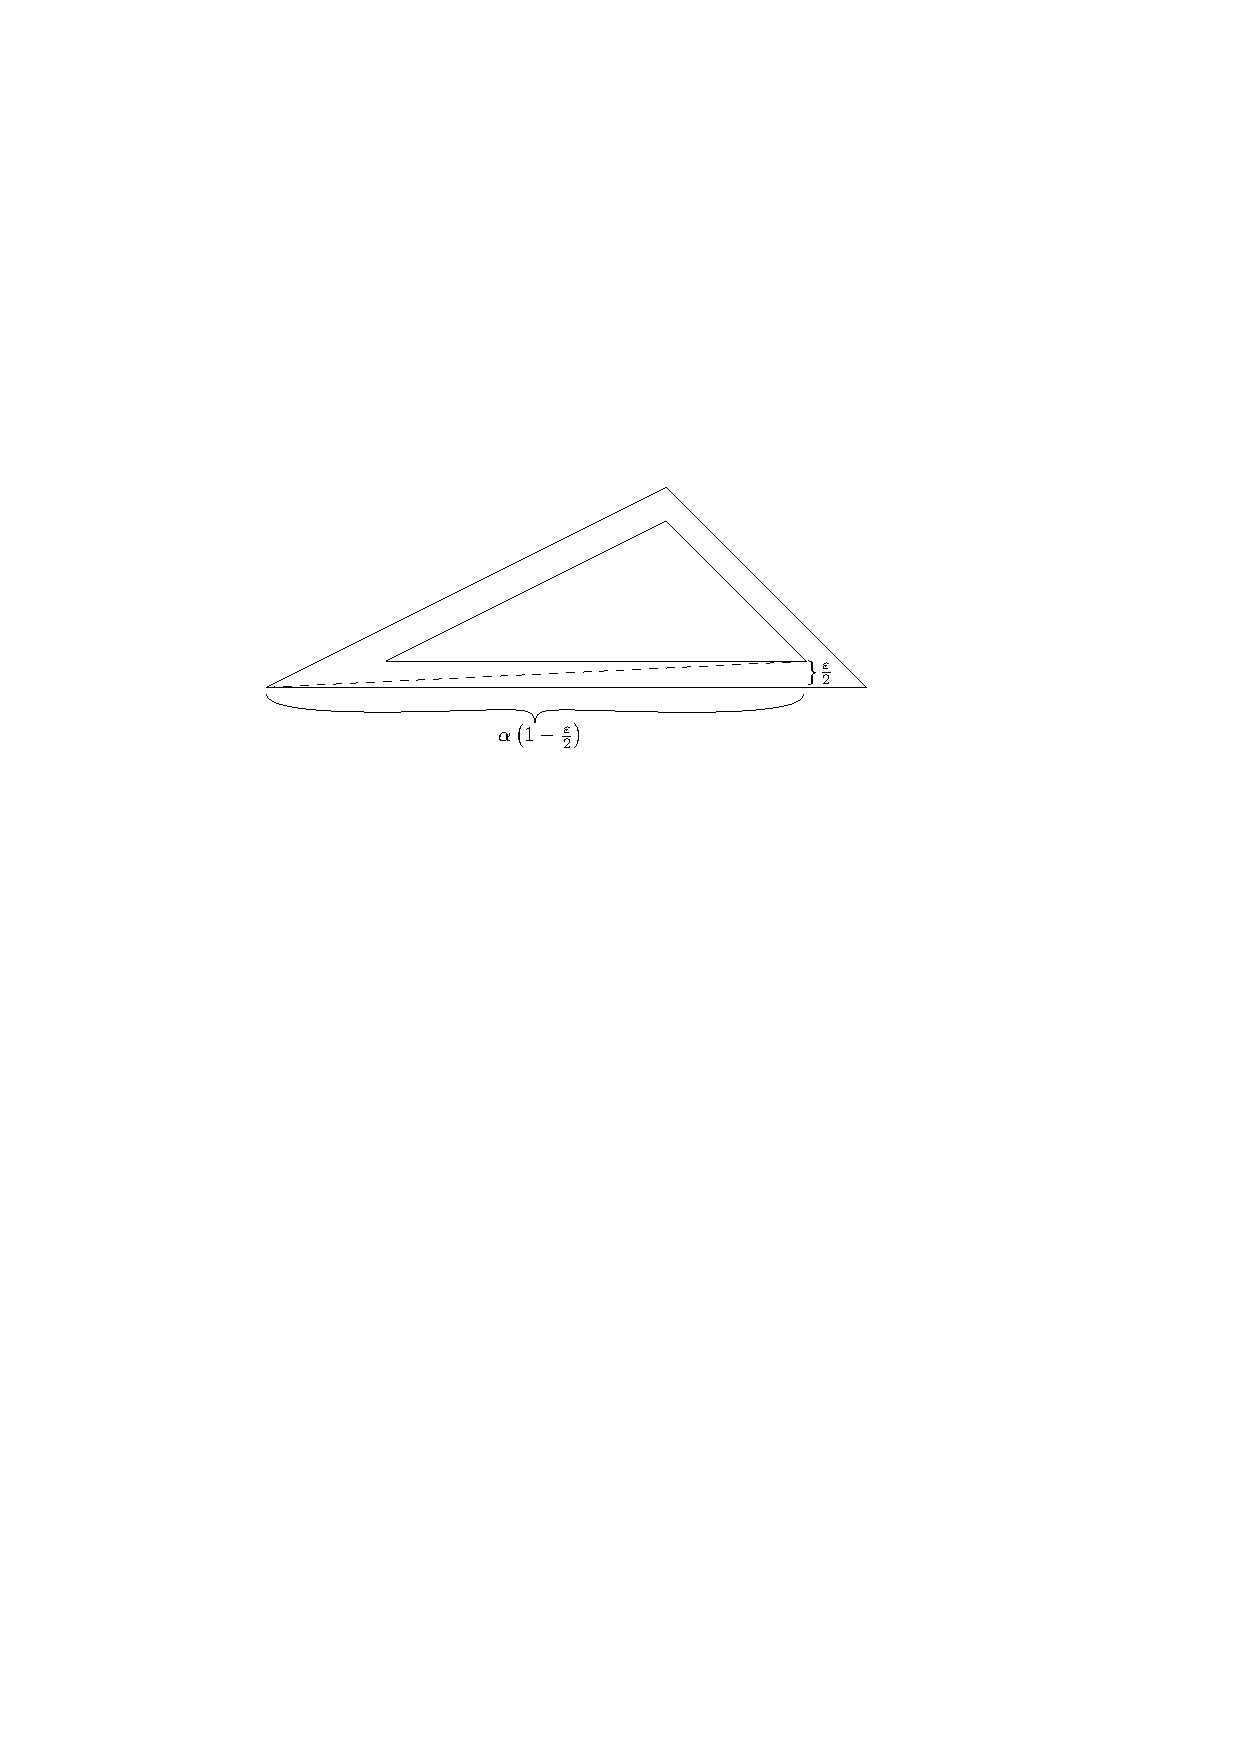
\includegraphics[width=0.6\linewidth]{figs/triangle_shadow}
    \figlab{triangle_with_shadow}
\end{figure}


\subsection{Fat convex regions}

Let $C$ be a convex shape, let $d_+$ be the smallest disk containing
$C$, and $d_-$ be the largest disk contained in $C$. We say that $C$
is $\alpha$-fat if the ratio $\frac{radius(d_+)}{radius(d_-)}$ is at
most $\alpha$. Let $\LL$ be the set of all $\alpha$-fat convex
shapes. In the following, we construct $(\LL, \eps)$-local
$t$-spanners for $t>1$.

We start by proving a structural lemma which will be later used in the
correctness proof.

\begin{claim}
    Let $C$ be an $\alpha$-fat convex shape, and let $C_{1-\eps}$ be
    the $\epsilon$ core of $C$. The shortest segment $\overline{pq}$
    such that $p,q\in\partial C$ and
    $\overline{pq}\cap C_{1-\eps}\neq \emptyset$ is of length at
    least %TO DO.
\end{claim}

\begin{proof}
    Let $d_-$ and $d_+$ be two disks, such that
    $d_-\subseteq C\subseteq d_+$, and
    $\frac{radius(d_+)}{radius(d_-)}=\alpha$, and let $\overline{pq}$
    be the a shortest segment. We assume
    $\overline{pq} \cap C_{1-\eps}$ is a single point $s$.
\end{proof}


\bibliographystyle{alpha}
% \bibliography{shortcuts,geometry}
\bibliography{ft_spanner}

\end{document}
